\pdfoutput=1 

\documentclass{article}

\usepackage{arxiv}
\usepackage{physics}
\usepackage{qcircuit}
\usepackage[utf8]{inputenc} % allow utf-8 input
\usepackage[T1]{fontenc}    % use 8-bit T1 fonts
\usepackage{hyperref}       % hyperlinks
\usepackage{url}            % simple URL typesetting
\usepackage{booktabs}       % professional-quality tables
\usepackage{amsfonts}       % blackboard math symbols
\usepackage{nicefrac}       % compact symbols for 1/2, etc.
\usepackage{microtype}      % microtypography
\usepackage{bbold}
\usepackage{subcaption}
%\usepackage{natbib}
%\usepackage{tikz}
%\usetikzlibrary{arrows.meta}
\usepackage{fullpage}
\usepackage{times}
\usepackage{enumitem}
\usepackage{fancyhdr,graphicx,amsmath,amssymb}
\usepackage{mathtools} % Loads amsmath
\usepackage[ruled,vlined]{algorithm2e}
%\usetikzlibrary{shapes.geometric, arrows}
\usepackage{nicefrac}
\usepackage{floatrow}
\usepackage{xparse}
%\usepackage[normalem]{ulem}
\usepackage{xcolor}
\newlength{\twosubht}
\newsavebox{\twosubbox}
\usepackage[titletoc,title]{appendix}

\usepackage{tabularx} %***
\usepackage{multirow}
% Table float box with bottom caption, box width adjusted to content


%\usepackage{blindtext}

\newcommand{\appendixhead}%
{\textbf{\huge Appendices}
\vspace{0.25in}}

\newfloatcommand{capbtabbox}{table}[][\FBwidth]

\definecolor{maiblue}{rgb}{0, 0., 0.69}
% \hypersetup{colorlinks=true, citecolor=maiblue, pdffitwindow=true, linkcolor=maiblue, urlcolor=maiblue}

\definecolor{Gray}{gray}{0.925}

\newcommand{\myrowcolour}{\rowcolor[gray]{0.925}}



\usepackage{graphicx}
\usepackage{tabularx} %***
\usepackage{multirow}
\usepackage{booktabs}
\usepackage[mode=math]{siunitx}
\usepackage{colortbl}
\usepackage{booktabs}
\usepackage{hyperref}



\definecolor{upforestgreen}{rgb}{0.0, 0.27, 0.13}
\newcommand{\highest}[1]{\textcolor{upforestgreen}{\textbf{$\bm{#1}$}}}%

\raggedbottom


\newcommand{\tens}[1]{%
  \mathbin{\mathop{\otimes}\displaylimits_{#1}}%
  }
\newcommand{\am}[1]{{\color{blue}{[{\textbf{AM}:} #1]}}}

\title{MAQA: A Quantum Framework for Supervised
Learning}
%\author{}


\author{
\href{https://orcid.org/0000-0002-1348-250X}{\includegraphics[scale=0.06]{orcid.pdf}\hspace{1mm}Antonio Macaluso}\thanks{corresponding author} \\
	German Research Center for Artificial Intelligence \\(DFKI)\\
	Saarbruecken, Germany\\
	\texttt{antonio.macaluso@dfki.de} \\
	\And
	%\href{https://orcid.org/0000-0000-0000-0000}\includegraphics[scale=0.06]{orcid.pdf}\hspace{1mm}
        Matthias Klusch \\ %}\\
	German Research Center for Artificial Intelligence \\(DFKI)\\
	Saarbruecken, Germany\\
	\texttt{matthias.klusch@dfki.de} \\
  \AND
      Stefano Lodi \\
    University of Bologna\\%   Mount-Sheikh University\\
    Bologna, Italy \\
    \texttt{stefano.lodi@unibo.it} \\
    \And
    Claudio Sartori \\
    University of Bologna\\%   Mount-Sheikh University\\
    Bologna, Italy \\
%   Santa Narimana, Levand \\
    \texttt{claudio.sartori@unibo.it} \\
  %% Coauthor \\
  %% Affiliation \\
  %% Address \\
  %% \texttt{email} \\
  %% \And
  %% Coauthor \\
  %% Affiliation \\
  %% Address \\
  %% \texttt{email} \\
  %% \And
  %% Coauthor \\
  %% Affiliation \\
  %% Address \\
  %% \texttt{email} \\
}





\begin{document}

\maketitle

\begin{abstract}
Quantum Machine Learning has the potential to improve traditional machine learning methods and overcome some of the main limitations imposed by the classical computing paradigm. However, the practical advantages of using quantum resources to solve pattern recognition tasks are still to be demonstrated.

This work proposes a universal, efficient framework that can reproduce the output of a plethora of classical supervised machine learning algorithms exploiting quantum computation's advantages. The proposed framework is named  \textit{Multiple Aggregator Quantum Algorithm} (MAQA) due to its capability to combine multiple and diverse functions to solve typical supervised learning problems. 
In its general formulation, MAQA can be potentially adopted as the quantum counterpart of all those models falling into the scheme of aggregation of multiple functions, such as ensemble algorithms and neural networks. From a computational point of view, the proposed framework allows generating an exponentially large number of different transformations of the input at the cost of increasing the depth of the corresponding quantum circuit linearly. Thus, MAQA produces a model with substantial descriptive power to broaden the horizon of possible applications of quantum machine learning with a computational advantage over classical methods. As a second meaningful addition, we discuss the adoption of the proposed framework as hybrid quantum-classical and fault-tolerant quantum algorithm.

\end{abstract}


% keywords can be removed
\keywords{Quantum Machine Learning \and Quantum Computing \and Machine Learning}


% \vspace{-10pt}
%%%%%%%%% BODY TEXT

\section{Introduction}
\label{section:introduction}
%% 1. why should someone care?

%The advent of advanced interactive computer vision systems~\cite{hololens} and recent progress in vision-language and multi-modal models~\cite{} opens doors for such next generation of assistive agents. 
% We envision that the future assistive agents would build up on these visual and language reasoning capabilities of today and empower users to achieve goals in their everyday lives. In particular, such agents would be able to reason about \emph{unseen} human goals... 
% We posit that such agents would require the ability to understand user goals described in natural language at high-level i.e., without complete details about as well as unseen user goals. 

%Recent progress in augmented reality systems~\cite{hololens, magicleap}, as well as vision-language and multi-modal models~\cite{}, opens doors for the next generation of assistive agents. 
Inspired by recent progress in visual systems~\cite{MagicLeap, ungureanu2020hololens}, we consider an assistive egocentric agent capable of reasoning about daily activities. When invoked via natural language commands, for e.g., while baking a cake, the agent understands the steps involved in baking, tracks progress through the various stages of the task, detects and proactively prevents mistakes by making suggestions. Such an agent would empower users to learn new skills and accomplish tasks efficiently.
% One could envision invoking such an agent merely through natural language descriptions of tasks similar to how present day assistants such as Alexa, Siri etc.~\cite{voice_assistants} are invoked. 
%We envision such agents to empower users in daily life by  invoking them naturally through 

%% 2. Why is it challenging? 
%While recent progress in vision-language and multi-modal models~\cite{} opens doors for such next generation of assistive agents, various challenges remain in making such agents a reality. 
%To make such agents a reality, 

Developing such an egocentric agent capable of tracking and verifying everyday tasks based on their natural language specification is challenging for multiple reasons. First, such an agent must reason about various ways of doing a \emph{multi-step} task specified in natural language. This entails decomposing the task into relevant actions, state changes, object interactions as well as any necessary causal and temporal relationships between these entities. Secondly, the agent must ground these entities in egocentric observations to track progress and detect mistakes. Lastly, to truly be useful, such an agent must support tracking and verification for a combination of tasks and, ideally, even unseen tasks. These three challenges -- causal and temporal reasoning about task structure from natural language, visual grounding of sub-tasks, and compositional generalization -- form the core goals of our work.

% %% 3. What are we doing? What is our approach?
% \aks{I think this is a matter of preference, but I personally don't like related work in intro. I would make this paragraph be about EgoTV and NSG. Starting with something like - "To this end, we propose...", ie, your next paragraph.}
% \nk{+1, we should move parts of this para to lit review and delete the rest.}
% Recent research on language modeling enables decomposing tasks into multiple steps from natural language descriptions~\cite{llm_zero_shot_planning,proscript}. However, such \emph{task decompositions} cannot directly be leveraged for task tracking in egocentric agents because of lack of grounding into the visual observations or context. In parallel, the computer vision community has advanced action recognition~\cite{}, object detection and tracking~\cite{}, hand object interaction and object state change detection~\cite{ego_4d,change_it,}, step classification in procedural tasks~\cite{}, and even vision language reasoning~\cite{nsvqa,nscl,star_situated_reasoning,clevrer}, which may help with the grounding challenge. However, majority of current research on identifying actions, objects, steps, or state changes does not account for the overall task structure. Likewise, predominant research on vision language understanding~\cite{} and multi-modal grounding~\cite{} does not consider the temporal and causal constraints that emerge in task tracking and verification. We therefore focus on the order-aware visual grounding problem in our work, with an eye towards compositional generalization to scale usability of these agents. In particular, we aim to achieve visual grounding of the actions and objects corresponding to each step or sub-task obtained from the task description decomposition in an order-aware manner.

%% 4. What are our results/contributions?
As our first contribution, we propose a benchmark -- \emph{\textbf{Ego}centric \textbf{T}ask \textbf{V}erification} (\etv \inlineimg{figures/TV}) -- and a corresponding dataset in the AI2-THOR~\cite{ai2thor} simulator. % \emoji{tv}
Given a natural language (NL) task description and a corresponding egocentric video of an agent, the goal of \etv is to verify whether the task was successfully completed in the video or not.
\etv contains multi-step tasks with \emph{ordering} constraints on the steps and \emph{abstracted} NL task descriptions with omitted low-level task details inspired by the needs of real-world assistants. We also provide splits of the dataset focused on different generalization aspects, e.g., unseen visual contexts, compositions of steps, and tasks (see Figure~\ref{figure:dataset}).
% Next, we create splits of the dataset focused on different aspects of generalization, ranging from generalization to unseen visual context to unseen compositions of steps and tasks. Figure~\ref{figure:dataset} shows an example task and overview of generalization splits from \etv. Succeeding at \etv tasks requires decomposing tasks into partially-ordered steps from the NL description and order-aware visual grounding of these steps into the video. 

Our second contribution is a novel approach for order-aware visual grounding~--~\emph{\textbf{N}euro-\textbf{S}ymbolic \textbf{G}rounding} (NSG), capable of compositional reasoning and generalizing to unseen tasks owing to its ability to leverage abstract NL descriptions and compositional structure of tasks (task decomposition, ordering).~In contrast, state-of-the-art vision-language models~\cite{coca,clip,videoclip,clip_hitchiker} struggle to ground NL descriptions in egocentric videos, and do not generalize to unseen tasks.~NSG outperforms these models by~$\mathbf{33.8}\%$~on compositional generalization and~$\mathbf{32.8}\%$~on abstractly described task verification. Finally, to evaluate \nsg on real-world data, we instantiate \etv on the CrossTask~\cite{cross_task} instructional video dataset. %Specifically, we synthetically create videos with mistakes in CrossTask. 
We find that it also outperforms state-of-the-art models at task verification on CrossTask. We hope that the \etv~benchmark and dataset will enable future research on egocentric agents capable of aiding in everyday tasks.

% We experiment with many for the \etv tasks. We find that while these models generalize well to unseen visual context, they struggle to perform grounding from abstracted task descriptions and to generalize to new compositions of tasks. To deal with these challenges, we take inspiration from recent research on and develop . ~\rd{unclear why neurosymbolic models would do well on abstraction.} 

% To summarize, our main contributions are:~1)~\etv: a benchmark and synthetic dataset to systematically study egocentric task verification.
% 2)~\nsg: a novel neuro-symbolic approach to enable the core reasoning capability for \etv -- order-aware visual grounding. We demonstrate \nsg's capability on our synthetic \etv dataset as well as a real-world dataset derived from CrossTask. We will release both of these datasets and our models for future research on egocentric task tracking and verification. 


% Assistive agents require the ability to track actions and state changes from an egocentric perspective for effective assistance in day-to-day tasks. For example, an agent helping a user prepare a recipe would need to both generate the steps of the recipe (\textit{plan generation}) and track the user's actions to ensure the plan is executed correctly (\textit{plan verification}). We formulate this as a Video Entailment task~\cite{violin_dataset,9710490} \rd{should we call our task video-based goal entailment?}, wherein, given an egocentric video of an agent (or human) performing a task (\textit{premise}) and a NL task description (\textit{hypothesis}), the objective is to learn a model to track whether the given task was successfully executed in the video. 
% An ideal model should also be able to seamlessly generalize to novel compositions (of actions and objects) unseen during training. \rd{add a line about what we mean by abstraction and why is it important.} To this end, we generate a novel Vision-Language dataset on the AI2-THOR simulator~\cite{ai2thor} to study compositional and abstraction-based generalization. Our dataset provides effective evaluation measures in a controlled setting, while closely reflecting the diversity of real-world events. We implement and train a variety of end-to-end models based on existing state-of-the-art approaches. We empirically demonstrate that neural models suffer from overfitting and cannot effectively generalize to novel compositions of actions, objects, and scenes. 
% To address this problem, we propose an end-to-end Neuro-Symbolic (NeSy) framework that performs plan generation and verification. At the heart of our approach is the hypothesis that symbolic reasoning models are good at generalization and capturing compositional substructure, while neural models are good at learning representations from sensory data~\cite{10.5555/3326943.3327039,nscl,clevrer}. \rd{summarize contributions in a bulleted list.} \rd{also add a line about the main result e.g., x\% improvement as compared to end-to-end models}. 

% \rd{we also evaluate NeSy with real-world data: add briefly about CrossTask experiments.}

% % \fbox{\begin{minipage}{\linewidth}
% % \textbf{Problem Statement}

% % Given:
% % (i) Premise: Egocentric video of an agent performing a task.
% % (ii) Hypothesis: NL description of the task.

% % Learn: A model to track whether the premise entails the hypothesis. The output of the model is True if the given task is executed successfully in the video.
% % \end{minipage}}

% \textbf{Contributions:} 
% \begin{itemize}
%     \item We generate a benchmark video-language dataset to study compositional and abstraction-based generalization.
%     \item We evaluate the performance of a variety of state-of-the-art models and show that these (baseline) models cannot effectively generalize to novel compositions of actions.
%     \item We propose a novel end-to-end NeSy approach that significantly outperforms the baselines on some compositional generalization splits while performing on par with them on the rest.
%     \item We also evaluate our NeSy approach with real-world data showing similar performance improvements.
% \end{itemize}

% \input{2_Background}
% \input{3_Quantum_Ensemble}
% \section{Application to the Example and Discussion}
\label{sec:discussion}

    This section proposes to illustrate the proposed transformation from AAF to action language for Example~\ref{ex:IRM_ou_radio}, highlighting its exploitation to get enriched information about the modelled dialogue, more precisely for providing visual representations justifying the acceptance or rejection of arguments. It considers successively two classes of argumentation explanations in \cite{cyras_survey}'s taxonomy: 
    it first shows how it can lead to graphical representations of the processes of accepting/rejecting arguments, it then discusses the case of causal explanations. 


        %In this section we apply program~$\Pi(\chi)$ to Example~\ref{ex:IRM_ou_radio}. The event trace $\tau_{\chi}^e$ and state trace~$\tau_{\chi}^s$, as well as the causal relations lead to Figures~\ref{fig:exemple_ini} and~\ref{fig:exemple_fin}.
        
    \subsection{Graphical Representation and Explanation}
    \label{sec:discu_temps}

    According to \cite{cyras_survey}, argumentation explanations can consist in extracting argumentative subgraphs to justify the acceptance or rejection of an argument for a given AAF semantics, producing a graphical representation of the underlying process.

% In argumentation, \cite{cyras_survey} proposed a classification of methods for generating explanations. Among them, one category focuses on the extraction of argumentative subgraphs to justify the acceptance or rejection of an argument for a certain semantics, producing a graphical representation of the process of accepting or rejecting an argument.
        
The transformation proposed in the previous section makes it possible to derive  graphical representations of the argumentative process. Indeed, the traces of events and states can be used  to obtain a narrative of the interaction that can be represented graphically. The visualisation we propose is illustrated in Figure~\ref{fig:exemple_ini}, in a simplified form, for Example~\ref{ex:IRM_ou_radio}. It is enriched in the next section using causality relations.


        \begin{figure}[t]
            \centering
        	\resizebox{7cm}{!}{

\tikzset{every picture/.style={line width=0.75pt}} %set default line width to 0.75pt        

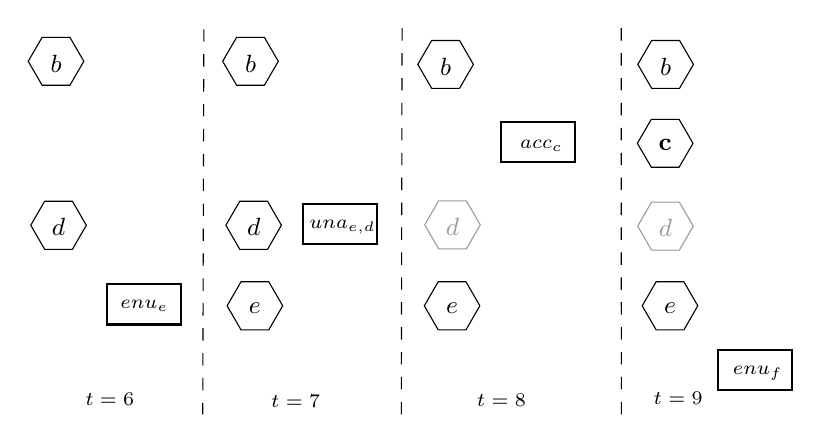
\begin{tikzpicture}[x=0.75pt,y=0.75pt,yscale=-1,xscale=1]
%uncomment if require: \path (0,300); %set diagram left start at 0, and has height of 300

%Shape: Rectangle [id:dp32394197299921523] 
\draw  [line width=0.75]  (38.8,129.2) -- (74.6,129.2) -- (74.6,148.54) -- (38.8,148.54) -- cycle ;
%Straight Lines [id:da5103454315814933] 
\draw  [dash pattern={on 4.5pt off 4.5pt}]  (85.53,6.3) -- (85,191.83) ;
%Straight Lines [id:da9625799604219181] 
\draw  [dash pattern={on 4.5pt off 4.5pt}]  (181.03,5.8) -- (180.67,191.83) ;
%Straight Lines [id:da937826652519754] 
\draw  [dash pattern={on 4.5pt off 4.5pt}]  (286.6,5.8) -- (286.67,191.83) ;
%Shape: Rectangle [id:dp39055029505322625] 
\draw  [line width=0.75]  (133.09,90.57) -- (168.89,90.57) -- (168.89,109.91) -- (133.09,109.91) -- cycle ;
%Shape: Polygon [id:dp25831662543105294] 
\draw   (27.7,21.73) -- (21,33.26) -- (7.6,33.26) -- (0.91,21.73) -- (7.6,10.19) -- (21,10.19) -- cycle ;
%Shape: Polygon [id:dp17264867524000027] 
\draw   (121.4,21.73) -- (114.7,33.26) -- (101.3,33.26) -- (94.6,21.73) -- (101.3,10.19) -- (114.7,10.19) -- cycle ;
%Shape: Polygon [id:dp9933858680624272] 
\draw   (215.4,23.23) -- (208.7,34.76) -- (195.3,34.76) -- (188.6,23.23) -- (195.3,11.69) -- (208.7,11.69) -- cycle ;
%Shape: Polygon [id:dp7138531738923998] 
\draw   (321.2,61.23) -- (314.5,72.76) -- (301.1,72.76) -- (294.4,61.23) -- (301.1,49.69) -- (314.5,49.69) -- cycle ;
%Shape: Regular Polygon [id:dp10291797427860683] 
\draw   (323.5,139.53) -- (316.81,151.12) -- (303.43,151.12) -- (296.74,139.53) -- (303.43,127.95) -- (316.81,127.95) -- cycle ;
%Shape: Regular Polygon [id:dp2894654570081998] 
\draw   (218.5,139.53) -- (211.81,151.12) -- (198.43,151.12) -- (191.74,139.53) -- (198.43,127.95) -- (211.81,127.95) -- cycle ;
%Shape: Regular Polygon [id:dp8293769486214224] 
\draw   (122.9,100.73) -- (116.21,112.32) -- (102.83,112.32) -- (96.14,100.73) -- (102.83,89.15) -- (116.21,89.15) -- cycle ;
%Shape: Regular Polygon [id:dp8361683320569804] 
\draw   (123.5,139.53) -- (116.81,151.12) -- (103.43,151.12) -- (96.74,139.53) -- (103.43,127.95) -- (116.81,127.95) -- cycle ;
%Shape: Regular Polygon [id:dp5470998290634859] 
\draw   (28.9,100.73) -- (22.21,112.32) -- (8.83,112.32) -- (2.14,100.73) -- (8.83,89.15) -- (22.21,89.15) -- cycle ;
%Shape: Rectangle [id:dp8416513794122603] 
\draw  [line width=0.75]  (228.69,50.97) -- (264.49,50.97) -- (264.49,70.31) -- (228.69,70.31) -- cycle ;
%Shape: Rectangle [id:dp842481801930145] 
\draw  [line width=0.75]  (333.09,160.97) -- (368.89,160.97) -- (368.89,180.31) -- (333.09,180.31) -- cycle ;
%Shape: Regular Polygon [id:dp0962459706720944] 
\draw  [color={rgb, 255:red, 155; green, 155; blue, 155 }  ,draw opacity=1 ] (218.7,100.53) -- (212.01,112.12) -- (198.63,112.12) -- (191.94,100.53) -- (198.63,88.95) -- (212.01,88.95) -- cycle ;
%Shape: Regular Polygon [id:dp5093510894708538] 
\draw  [color={rgb, 255:red, 155; green, 155; blue, 155 }  ,draw opacity=1 ] (321.3,101.13) -- (314.61,112.72) -- (301.23,112.72) -- (294.54,101.13) -- (301.23,89.55) -- (314.61,89.55) -- cycle ;
%Shape: Polygon [id:dp3364030899411299] 
\draw   (321.4,23.23) -- (314.7,34.76) -- (301.3,34.76) -- (294.6,23.23) -- (301.3,11.69) -- (314.7,11.69) -- cycle ;

% Text Node
\draw (27.13,180.4) node [anchor=north west][inner sep=0.75pt]  [font=\scriptsize]  {$t=6$};
% Text Node
\draw (44,135.6) node [anchor=north west][inner sep=0.75pt]  [font=\scriptsize]  {$enu_{e}$};
% Text Node
\draw (135.09,96.97) node [anchor=north west][inner sep=0.75pt]  [font=\scriptsize]  {$una_{e,d}$};
% Text Node
\draw (116.67,181.33) node [anchor=north west][inner sep=0.75pt]  [font=\scriptsize]  {$t=7$};
% Text Node
\draw (215.8,180.9) node [anchor=north west][inner sep=0.75pt]  [font=\scriptsize]  {$t=8$};
% Text Node
\draw (301,179.9) node [anchor=north west][inner sep=0.75pt]  [font=\scriptsize]  {$t=9$};
% Text Node
\draw (14.3,22.73) node  [font=\small]  {$b$};
% Text Node
\draw (108,22.73) node  [font=\small]  {$b$};
% Text Node
\draw (202,24.23) node  [font=\small]  {$b$};
% Text Node
\draw (307.8,62.23) node  [font=\small]  {$\mathbf{c}$};
% Text Node
\draw (310.12,140.53) node  [font=\small]  {$e$};
% Text Node
\draw (205.12,140.53) node  [font=\small]  {$e$};
% Text Node
\draw (109.52,101.73) node  [font=\small]  {$d$};
% Text Node
\draw (110.12,140.53) node  [font=\small]  {$e$};
% Text Node
\draw (15.52,101.73) node  [font=\small]  {$d$};
% Text Node
\draw (236.69,58.57) node [anchor=north west][inner sep=0.75pt]  [font=\scriptsize]  {$acc_{c}$};
% Text Node
\draw (339.09,167.57) node [anchor=north west][inner sep=0.75pt]  [font=\scriptsize]  {$enu_{f}$};
% Text Node
\draw (205.32,101.53) node  [font=\small,color={rgb, 255:red, 155; green, 155; blue, 155 }  ,opacity=1 ]  {$d$};
% Text Node
\draw (307.92,102.13) node  [font=\small,color={rgb, 255:red, 155; green, 155; blue, 155 }  ,opacity=1 ]  {$d$};
% Text Node
\draw (308,24.23) node  [font=\small]  {$b$};


\end{tikzpicture}
}
        	\caption{Partial graphical representation 
        	%of event and state traces $\tau_{\chi}^e$ and $\tau_{\chi}^s$ 
        	associated to Example~\ref{ex:IRM_ou_radio}. 
        	Hexagons represent fluents and rectangles events.
        	}
        	\label{fig:exemple_ini} 
        \end{figure}

        \begin{table}[t]
        \footnotesize
        \addtolength{\tabcolsep}{-1pt}
        \begin{center}
            \begin{tabular}{|c|cccccccccccc|c|}
        % \hline
        %  & \multicolumn{13}{c|}{Séquence d'action $enunciate_x$} \\ \cline{2-14}
        \hline
         & $a$ & \multicolumn{1}{|c|}{$b$} & \multicolumn{1}{c|}{$c$} & \multicolumn{1}{c|}{$d$} & \multicolumn{1}{c|}{$e$} & \multicolumn{1}{c|}{$f$} & \multicolumn{1}{c|}{$g$} & \multicolumn{1}{c|}{$h$,$i$} & \multicolumn{1}{c|}{$j$} & \multicolumn{1}{c|}{$k$} & \multicolumn{1}{c|}{$l$} & $m$ & $n$ \\ \hline
        $a$ & \multicolumn{1}{c|}{\scriptsize{$\bullet$}} & \multicolumn{1}{c|}{\scriptsize{$\circ$}} & \multicolumn{1}{c|}{\scriptsize{$\circ$}} & \multicolumn{1}{c|}{\scriptsize{$\circ$}} & \multicolumn{1}{c|}{\scriptsize{$\circ$}} & \multicolumn{1}{c|}{\scriptsize{$\circ$}} & \multicolumn{1}{c|}{\scriptsize{$\circ$}} & \multicolumn{1}{c|}{\scriptsize{$\circ$}} & \multicolumn{1}{c|}{\scriptsize{$\circ$}} & \multicolumn{1}{c|}{\scriptsize{$\circ$}} & \multicolumn{1}{c|}{\scriptsize{$\circ$}} & \scriptsize{$\circ$} & \scriptsize{$\circ$} \\ \hline
        $b$ & \multicolumn{1}{c|}{\cellcolor[HTML]{B2BEB5}} & \multicolumn{1}{c|}{\scriptsize{$\bullet$}} & \multicolumn{1}{c|}{\scriptsize{$\bullet$}} & \multicolumn{1}{c|}{\scriptsize{$\bullet$}} & \multicolumn{1}{c|}{\scriptsize{$\bullet$}} & \multicolumn{1}{c|}{\scriptsize{$\bullet$}} & \multicolumn{1}{c|}{\scriptsize{$\bullet$}} & \multicolumn{1}{c|}{\scriptsize{$\bullet$}} & \multicolumn{1}{c|}{\scriptsize{$\bullet$}} & \multicolumn{1}{c|}{\scriptsize{$\bullet$}} & \multicolumn{1}{c|}{\scriptsize{$\bullet$}} & \scriptsize{$\bullet$} & \scriptsize{$\bullet$} \\ \cline{1-1} \cline{3-14} 
        $c$ & \cellcolor[HTML]{B2BEB5} & \multicolumn{1}{c|}{\cellcolor[HTML]{B2BEB5}} & \multicolumn{1}{c|}{\scriptsize{$\bullet$}} & \multicolumn{1}{c|}{\scriptsize{$\circ$}} & \multicolumn{1}{c|}{\scriptsize{$\bullet$}} & \multicolumn{1}{c|}{\scriptsize{$\circ$}} & \multicolumn{1}{c|}{\scriptsize{$\bullet$}} & \multicolumn{1}{c|}{\scriptsize{$\circ$}} & \multicolumn{1}{c|}{\scriptsize{$\circ$}} & \multicolumn{1}{c|}{\scriptsize{$\bullet$}} & \multicolumn{1}{c|}{\scriptsize{$\bullet$}} & \scriptsize{$\bullet$} & \scriptsize{$\circ$} \\ \cline{1-1} \cline{4-14} 
        $d$ & \cellcolor[HTML]{B2BEB5} & \cellcolor[HTML]{B2BEB5} & \multicolumn{1}{c|}{\cellcolor[HTML]{B2BEB5}} & \multicolumn{1}{c|}{\scriptsize{$\bullet$}} & \multicolumn{1}{c|}{\scriptsize{$\circ$}} & \multicolumn{1}{c|}{\scriptsize{$\bullet$}} & \multicolumn{1}{c|}{\scriptsize{$\circ$}} & \multicolumn{1}{c|}{\scriptsize{$\circ$}} & \multicolumn{1}{c|}{\scriptsize{$\circ$}} & \multicolumn{1}{c|}{\scriptsize{$\circ$}} & \multicolumn{1}{c|}{\scriptsize{$\circ$}} & \scriptsize{$\circ$} & \scriptsize{$\circ$} \\ \cline{1-1} \cline{5-14} 
        $e$ & \cellcolor[HTML]{B2BEB5} & \cellcolor[HTML]{B2BEB5} & \cellcolor[HTML]{B2BEB5} & \multicolumn{1}{c|}{\cellcolor[HTML]{B2BEB5}} & \multicolumn{1}{c|}{\scriptsize{$\bullet$}} & \multicolumn{1}{c|}{\scriptsize{$\circ$}} & \multicolumn{1}{c|}{\scriptsize{$\bullet$}} & \multicolumn{1}{c|}{\scriptsize{$\bullet$}} & \multicolumn{1}{c|}{\scriptsize{$\bullet$}} & \multicolumn{1}{c|}{\scriptsize{$\bullet$}} & \multicolumn{1}{c|}{\scriptsize{$\bullet$}} & \scriptsize{$\bullet$} & \scriptsize{$\bullet$} \\ \cline{1-1} \cline{6-14} 
        $f$ & \cellcolor[HTML]{B2BEB5} & \cellcolor[HTML]{B2BEB5} & \cellcolor[HTML]{B2BEB5} & \cellcolor[HTML]{B2BEB5} & \multicolumn{1}{c|}{\cellcolor[HTML]{B2BEB5}} & \multicolumn{1}{c|}{\scriptsize{$\bullet$}} & \multicolumn{1}{c|}{\scriptsize{$\circ$}} & \multicolumn{1}{c|}{\scriptsize{$\circ$}} & \multicolumn{1}{c|}{\scriptsize{$\circ$}} & \multicolumn{1}{c|}{\scriptsize{$\circ$}} & \multicolumn{1}{c|}{\scriptsize{$\circ$}} & \scriptsize{$\circ$} & \scriptsize{$\circ$} \\ \cline{1-1} \cline{7-14} 
        $g$ & \cellcolor[HTML]{B2BEB5} & \cellcolor[HTML]{B2BEB5} & \cellcolor[HTML]{B2BEB5} & \cellcolor[HTML]{B2BEB5} & \cellcolor[HTML]{B2BEB5} & \multicolumn{1}{c|}{\cellcolor[HTML]{B2BEB5}} & \multicolumn{1}{c|}{\scriptsize{$\bullet$}} & \multicolumn{1}{c|}{\scriptsize{$\bullet$}} & \multicolumn{1}{c|}{\scriptsize{$\bullet$}} & \multicolumn{1}{c|}{\scriptsize{$\bullet$}} & \multicolumn{1}{c|}{\scriptsize{$\bullet$}} & \scriptsize{$\bullet$} & \scriptsize{$\bullet$} \\ \cline{1-1} \cline{8-14} 
        $h$ & \cellcolor[HTML]{B2BEB5} & \cellcolor[HTML]{B2BEB5} & \cellcolor[HTML]{B2BEB5} & \cellcolor[HTML]{B2BEB5} & \cellcolor[HTML]{B2BEB5} & \cellcolor[HTML]{B2BEB5} & \multicolumn{1}{c|}{\cellcolor[HTML]{B2BEB5}} & \multicolumn{1}{c|}{\scriptsize{$\bullet$}} & \multicolumn{1}{c|}{\scriptsize{$\circ$}} & \multicolumn{1}{c|}{\scriptsize{$\circ$}} & \multicolumn{1}{c|}{\scriptsize{$\circ$}} & \scriptsize{$\circ$} & \scriptsize{$\circ$} \\ \cline{1-1} \cline{9-14} 
        $i$ & \cellcolor[HTML]{B2BEB5} & \cellcolor[HTML]{B2BEB5} & \cellcolor[HTML]{B2BEB5} & \cellcolor[HTML]{B2BEB5} & \cellcolor[HTML]{B2BEB5} & \cellcolor[HTML]{B2BEB5} & \multicolumn{1}{c|}{\cellcolor[HTML]{B2BEB5}} & \multicolumn{1}{c|}{\scriptsize{$\bullet$}} & \multicolumn{1}{c|}{\scriptsize{$\bullet$}} & \multicolumn{1}{c|}{\scriptsize{$\circ$}} & \multicolumn{1}{c|}{\scriptsize{$\circ$}} & \scriptsize{$\circ$} & \scriptsize{$\circ$} \\ \cline{1-1} \cline{9-14} 
        $j$ & \cellcolor[HTML]{B2BEB5} & \cellcolor[HTML]{B2BEB5} & \cellcolor[HTML]{B2BEB5} & \cellcolor[HTML]{B2BEB5} & \cellcolor[HTML]{B2BEB5} & \cellcolor[HTML]{B2BEB5} & \cellcolor[HTML]{B2BEB5} & \multicolumn{1}{c|}{\cellcolor[HTML]{B2BEB5}} & \multicolumn{1}{c|}{\scriptsize{$\bullet$}} & \multicolumn{1}{c|}{\scriptsize{$\bullet$}} & \multicolumn{1}{c|}{\scriptsize{$\bullet$}} & \scriptsize{$\bullet$} & \scriptsize{$\bullet$} \\ \cline{1-1} \cline{10-14} 
        $k$ & \cellcolor[HTML]{B2BEB5} & \cellcolor[HTML]{B2BEB5} & \cellcolor[HTML]{B2BEB5} & \cellcolor[HTML]{B2BEB5} & \cellcolor[HTML]{B2BEB5} & \cellcolor[HTML]{B2BEB5} & \cellcolor[HTML]{B2BEB5} & \cellcolor[HTML]{B2BEB5} & \multicolumn{1}{c|}{\cellcolor[HTML]{B2BEB5}} & \multicolumn{1}{c|}{\scriptsize{$\bullet$}} & \multicolumn{1}{c|}{\scriptsize{$\bullet$}} & \scriptsize{$\bullet$} & \scriptsize{$\bullet$} \\ \cline{1-1} \cline{11-14} 
        $l$ & \cellcolor[HTML]{B2BEB5} & \cellcolor[HTML]{B2BEB5} & \cellcolor[HTML]{B2BEB5} & \cellcolor[HTML]{B2BEB5} & \cellcolor[HTML]{B2BEB5} & \cellcolor[HTML]{B2BEB5} & \cellcolor[HTML]{B2BEB5} & \cellcolor[HTML]{B2BEB5} & \cellcolor[HTML]{B2BEB5} & \multicolumn{1}{c|}{\cellcolor[HTML]{B2BEB5}} & \multicolumn{1}{c|}{\scriptsize{$\bullet$}} & \scriptsize{$\circ$} & \scriptsize{$\bullet$} \\ \cline{1-1} \cline{12-14} 
        $m$ & \cellcolor[HTML]{B2BEB5} & \cellcolor[HTML]{B2BEB5} & \cellcolor[HTML]{B2BEB5} & \cellcolor[HTML]{B2BEB5} & \cellcolor[HTML]{B2BEB5} & \cellcolor[HTML]{B2BEB5} & \cellcolor[HTML]{B2BEB5} & \cellcolor[HTML]{B2BEB5} & \cellcolor[HTML]{B2BEB5} & \cellcolor[HTML]{B2BEB5} & \multicolumn{1}{c|}{\cellcolor[HTML]{B2BEB5}} & \scriptsize{$\bullet$} & \scriptsize{$\circ$} \\ \cline{1-1} \cline{13-14} 
        $n$ & \cellcolor[HTML]{B2BEB5} & \cellcolor[HTML]{B2BEB5} & \cellcolor[HTML]{B2BEB5} & \cellcolor[HTML]{B2BEB5} & \cellcolor[HTML]{B2BEB5} & \cellcolor[HTML]{B2BEB5} & \cellcolor[HTML]{B2BEB5} & \cellcolor[HTML]{B2BEB5} & \cellcolor[HTML]{B2BEB5} & \cellcolor[HTML]{B2BEB5} & \cellcolor[HTML]{B2BEB5} & \cellcolor[HTML]{B2BEB5} & \scriptsize{$\bullet$} \\ \hline
        \end{tabular}
        \end{center}
        \caption{Tabular representation of the entire interaction.        
        \label{tab:scenario1}}
        \end{table}
        
        Given an event and a state traces~$\tau_{\chi}^e$ and~$\tau_{\chi}^s$, we propose to display the consecutive states, showing fluents as hexagons and the triggered events as rectangles. Since the acceptability of arguments is %what is mainly observed,
        what mainly matters, we propose to represent only the fluents $a_x$, using the argument names for the sake of readability.  
        Moreover, we do not show fluents when their negation is true in the state, except when the occurrence of a represented event results in the negation of the fluent. In this case, the negation is represented by a lighter shade. The events~$enunciate_x$, $makesUnacc_{y,x}$, and~$makesAcc_x$ are shortened as~$enu_x$, $una_{y,x}$, and~$acc_x$, respectively.
        

        \addtocounter{example}{-1}
        \begin{example} (continued) --
            Figure~\ref{fig:exemple_ini} shows a partial representation of the state trace obtained for Example~\ref{ex:IRM_ou_radio} using the ASP implementation described in Section~\ref{sec:ASP}. 
            
            The first represented state corresponds to~$S(6)$, an argumentative state in the sense of Def.~\ref{def:admissible_state}, which allows for the enunciation of the next argument: since all arguments preceding~$e$ have already been enunciated, the action~$enunciate_e$ can be performed. The occurrence of this event is the transition to the next state~$S(7)$ where, as shown in Figure~\ref{fig:exemple_ini}, argument~$e$ is acceptable. Unlike~$S(6)$, $S(7)$ is not an argumentative state: condition (i) of Def.~\ref{def:admissible_state} is not satisfied because~${(a_d\wedge cA_{e,d})}$ and~${a_e\in S(7)}$. Therefore, the next argument cannot be enunciated. However, since the triggering conditions of~$makesUnacc_{e,d}$ are satisfied, this exogenous event is triggered, leading to a new state transition. Since argument $d$ is no longer acceptable in~$S(8)$, condition (i)  of Def.~\ref{def:admissible_state} is now satisfied. Still, condition (ii) is not satisfied by~$S(8)$, preventing the next argument from being enunciated. Instead,~$makesAcc_c$ is triggered, leading to the following state~$S(9)$. Here, as shown in Figure~\ref{fig:exemple_ini}, argument~$c$ is acceptable. As this new state is argumentative, the next argument,~$f$, can be stated. The dialogue continues step by step and ends at state~$S(31)$. 
        \end{example}
        

        A second, more compact, tabular visualisation is proposed, illustrated in Table~\ref{tab:scenario1}: the arguments are represented in the first column, the order of the performed actions in the first row. For the sake of readability,  $enunciate_x$ is shortened as~$x$. In each table cell, $\bullet$ means that the argument is acceptable while~$\circ$ means that it is not. If an argument has not been enunciated yet, its acceptability cannote be evaluated, which is represented by the shaded boxes. In contrast to the previous representation where the updating stages are shown, this second form has the advantage of being more compact and allows the display the whole dialogue. It also makes it possible to  see quickly the direct and indirect impacts of the argument enunciation on the other argument acceptability. In particular, the enunciation order effect can be observed, as illustrated by the graphical comparison of Example~\ref{ex:IRM_ou_radio} and its modification given in Example~\ref{ex:IRM_ou_radio_modif}.
        
        \begin{example}\label{ex:IRM_ou_radio_modif}
          Let us consider the same dialogue as in Example~\ref{ex:IRM_ou_radio}, starting with the enunciation of arguments $a,b,c$, but considering that the physician then directly asks if it is possible to do the MRI today ($l$). The radiologist replies that he can only do it in two days at the earliest~($m$). The physician then specifies that it is an emergency~($n$). The remaining arguments are then enunciated in the same order ad in the initial example.
          
          Table~\ref{tab:scenario2} displays the proposed compact visualisation  for the evolution of the acceptability of the decision variable~$c$, starting from its enunciation. Even if the final state of the argumentation graph is identical, as expected according to Proposition~\ref{prop:indep_order} established in the previous section,
          with~$c$ being rejected, the display makes it easy to observe the very important impact that the order of the actions can have on the intermediate stages that lead to it: in the new scenario,~$c$ is not accepted from the $6^{th}$~action, i.e. $n$~enunciation, with no modification until the end.  
        \end{example}
        
        This visualisation thus also illustrates the relevance of the temporality integration in the argumentation framework: the differences between the two scenarios cannot be captured by classical AAFs. 
        
        \begin{table}[t]
            \addtolength{\tabcolsep}{-1pt}
            \begin{center}
                \begin{tabular}{|c|c|c|c|c|c|c|c|c|c|c|c|}
                \hline
                $\varsigma_1$ &  c & d & e & f & g & h,i & j & k & l & m & n \\ \hline
                c & \scriptsize{$\bullet$} & \scriptsize{$\circ$} & \scriptsize{$\bullet$} & \scriptsize{$\circ$} & \scriptsize{$\bullet$} & \scriptsize{$\circ$} & \scriptsize{$\circ$} & \scriptsize{$\bullet$} & \scriptsize{$\bullet$} & \scriptsize{$\bullet$} & \scriptsize{$\circ$} \\ 
                \hhline{|=|=|=|=|=|=|=|=|=|=|=|=|} 
                % \hline \hline
                $\varsigma_2$ & c & l & m & n & d & e & f & g & h,i & j & k \\ \hline
                c & \scriptsize{$\bullet$} & \scriptsize{$\bullet$} & \scriptsize{$\bullet$} & \scriptsize{$\circ$} & \scriptsize{$\circ$} & \scriptsize{$\circ$} & \scriptsize{$\circ$} & \scriptsize{$\circ$} & \scriptsize{$\circ$} & \scriptsize{$\circ$} & \scriptsize{$\circ$} \\ \hline
                \end{tabular}
            \end{center}           
            \caption{Impact of the order in which arguments are enunciated~(lines 1, 3) on the acceptability of the arguments~(lines 2, 4).\vspace{-2mm}}
            \label{tab:scenario2}
        \end{table}
        
    \subsection{On Causality and Explanation}
    \label{sec:discu_causalite}
    
    Beyond the graphical representation of the acceptance/rejection process, the proposed formalisation of AAF into action models provides tools for richer explanations, allowing us to transfer the notion of actual causality recalled in Section~\ref{sec:causality} to the argumentation framework. Indeed, the extraction of causal chains  has been shown to be an important property for explanations~\cite{miller_explanation_2018}. In the taxonomy proposed in the case of argumentation in \cite{cyras_survey}, such a causal explanation can be related to the identification of arguments that must be removed from an argumentation graph to make a non-acceptable argument acceptable~\cite{fan2015explanations}. In causal terminology, this corresponds to the search for a \textit{but-for} cause of the non-acceptability of an argument. 
    %\mj{qui pour moi a un côté contrastif, non ?} \Camu{je pense que oui, mais Yann est l'expert dans le domaine} \mj{on lui demandera demain}
    
    However, this test does not solve cases where the occurrence of one of two events would have been sufficient to cause an effect in the absence of the other, called over-determination~\cite{menzies_counterfactual_2020}. Among others, the definition of causality underlying the NESS test, as briefly recalled in Section~\ref{sec:causality} and implemented for the considered action language, makes it possible to solve this issue. 
    
    
    %\mj{coupe à la hache !!! plus rien sur les équations structurelles et le modèle de Halpern, ce qui est très violent. En même temps, je medemande pourquoi on discute de la différence entre la causalité à la Halpern et celle à la NESS ici ? Parce qu'il a été propos (par Yann) de représenter les graphes argumentatifs en graphes cauaux ? OK, alors je vais tâcher de les réintéger, en version courte}
    Structural equations~\cite{halpern2005causes} constitute another formal model of causality that addresses the over-determination issue and can be exploited in the argumentation framework, using the transformation of acyclic abstract argumentation graphs to that formalism proposed in~\cite{munro2022argumentation}. The main differences are as follows: from a philosophical point of view, the definition of causality underlying the NESS test belongs to the family of regularity approaches~\cite{andreas_regularity_2021}, whereas Halpern's definitions belong to the family of counterfactual approaches~\cite{menzies_counterfactual_2020}. Secondly, the use of action languages makes it possible to model and take into account temporality and the dynamics of the dialogue, which is a crucial component. From a mathematical point of view, according to~\cite{beckers_causal_2021}, Halpern's definition of causality can be described as `Contrastive actual weak sufficiency', whereas the one used here would be `Minimal actual strong sufficiency': in a nutshell, whereas the former emphasises that a cause must be necessary for an effect, hence the contrastive aspect, the latter emphasises sufficiency and subordinates necessity to it. From a practical point of view, the advantage of the causal approach used here is that it does not require counterfactual reasoning or interventionism, mechanisms that are computationally onerous and criticised for introducing subjectivity into causal enquiry~\cite{sarmiento_action_2022-1,wright_causation_1985}. 
    
    
    
    
    %To solve this issue, other methods must be used, such as the one presented in  Section~\ref{sec:causality} or the structural equations of~\cite{halpern2005causes}. Although these two methods make it possible to deal with cases of over-determination, they are not doing it in the same way and do not agree on the same result. From a philosophical point of view, the definition of causality underlying the NESS test belongs to the family of regularity approaches~\cite{andreas_regularity_2021}, whereas Halpern's definitions belong to the family of counterfactual approaches~\cite{menzies_counterfactual_2020}. Resolving the debate on which approach is more adequate is outside the scope of this article. \cite{munro2022argumentation} propose a transformation of acyclic abstract argumentation graphs to exploit Halpern's latest definition of causality to generate causal explanations in argumentation. Let us explain the main differences.
        
    %The first difference lies in the way we represent the world. Indeed, as shown in Section~\ref{sec:discu_temps}, the use of an action language allows us to take into account the dynamics of the dialogue. This is not negligible for understanding the latter, given that temporality seems to be fundamental to how we represent the world. The second difference is related to causality. From a purely mathematical point of view, Halpern's definition of causality can be described as "Contrastive actual weak sufficiency" according to~\cite{beckers_causal_2021}, whereas the one used here would be "Minimal actual strong sufficiency" according to this same typology. \Camu{In a nutshell, whereas the former emphasises that a cause must be necessary for an effect, hence the contrastive aspect, the latter emphasises sufficiency and subordinates necessity to it.} For more details on the implications of these differences, see~\cite{beckers_causal_2021,wright_causation_1985,wright_ness_2011}. \Camu{From a practical point of view, the advantage of the causal approach used here is that it does not require counterfactual reasoning or interventionism, mechanisms that are computationally onerous and criticised for introducing subjectivity into causal enquiry~\cite{sarmiento_action_2022-1,wright_causation_1985}. The fact that the causal analysis is carried out a posteriori, i.e. with full knowledge of the course of events, deprives counterfactual methods of their advantage, which are very useful when reasoning a priori and wanting to explore other possible courses of action.}
    

        These causal relations, that may lead later to causal explanations,
        %\Yann{Relation non ? Ce ne sont pas encore vraiment des explications} 
        can be represented graphically, enriching the proposed  visualisation illustrated in Figure~\ref{fig:exemple_ini} by different types of causes. This principle is illustrated in Figure~\ref{fig:exemple_fin}, commented below. 
        
        \begin{figure}[t]
            \centering
        	\resizebox{7cm}{!}{

\tikzset{every picture/.style={line width=0.75pt}} %set default line width to 0.75pt        

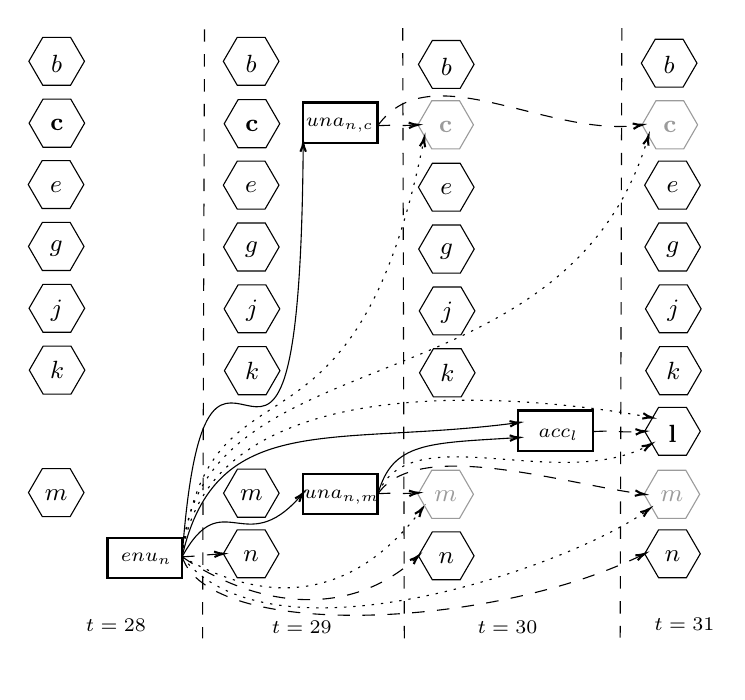
\begin{tikzpicture}[x=0.75pt,y=0.75pt,yscale=-1,xscale=1]
%uncomment if require: \path (0,300); %set diagram left start at 0, and has height of 300

%Shape: Rectangle [id:dp32394197299921523] 
\draw  [line width=0.75]  (38.8,251.2) -- (74.6,251.2) -- (74.6,270.54) -- (38.8,270.54) -- cycle ;
%Straight Lines [id:da5103454315814933] 
\draw  [dash pattern={on 4.5pt off 4.5pt}]  (85.53,6.3) -- (84.6,299.8) ;
%Straight Lines [id:da9625799604219181] 
\draw  [dash pattern={on 4.5pt off 4.5pt}]  (181.03,5.8) -- (181.8,299.8) ;
%Straight Lines [id:da937826652519754] 
\draw  [dash pattern={on 4.5pt off 4.5pt}]  (286.6,5.8) -- (285.8,299.4) ;
%Shape: Rectangle [id:dp39055029505322625] 
\draw  [line width=0.75]  (133.09,41.57) -- (168.89,41.57) -- (168.89,60.91) -- (133.09,60.91) -- cycle ;
%Shape: Polygon [id:dp25831662543105294] 
\draw   (27.7,21.73) -- (21,33.26) -- (7.6,33.26) -- (0.91,21.73) -- (7.6,10.19) -- (21,10.19) -- cycle ;
%Shape: Polygon [id:dp17264867524000027] 
\draw   (121.4,21.73) -- (114.7,33.26) -- (101.3,33.26) -- (94.6,21.73) -- (101.3,10.19) -- (114.7,10.19) -- cycle ;
%Shape: Polygon [id:dp9933858680624272] 
\draw   (215.4,23.23) -- (208.7,34.76) -- (195.3,34.76) -- (188.6,23.23) -- (195.3,11.69) -- (208.7,11.69) -- cycle ;
%Shape: Rectangle [id:dp8416513794122603] 
\draw  [line width=0.75]  (236.69,189.97) -- (272.49,189.97) -- (272.49,209.31) -- (236.69,209.31) -- cycle ;
%Curve Lines [id:da03689428077806867] 
\draw  [dash pattern={on 4.5pt off 4.5pt}]  (74.74,260.46) .. controls (110.24,284.75) and (154.9,290.88) .. (187.62,260.92) ;
\draw [shift={(188.6,260)}, rotate = 136.62] [color={rgb, 255:red, 0; green, 0; blue, 0 }  ][line width=0.75]    (4.37,-1.32) .. controls (2.78,-0.56) and (1.32,-0.12) .. (0,0) .. controls (1.32,0.12) and (2.78,0.56) .. (4.37,1.32)   ;
%Curve Lines [id:da9511759619364188] 
\draw    (74.74,260.46) .. controls (94.3,224.74) and (104.69,262.24) .. (131.75,231.26) ;
\draw [shift={(133,229.8)}, rotate = 129.81] [color={rgb, 255:red, 0; green, 0; blue, 0 }  ][line width=0.75]    (4.37,-1.32) .. controls (2.78,-0.56) and (1.32,-0.12) .. (0,0) .. controls (1.32,0.12) and (2.78,0.56) .. (4.37,1.32)   ;
%Shape: Regular Polygon [id:dp0962459706720944] 
\draw  [color={rgb, 255:red, 155; green, 155; blue, 155 }  ,draw opacity=1 ] (215.1,52.33) -- (208.41,63.92) -- (195.03,63.92) -- (188.34,52.33) -- (195.03,40.75) -- (208.41,40.75) -- cycle ;
%Curve Lines [id:da23781812589748064] 
\draw  [dash pattern={on 0.84pt off 2.51pt}]  (74.74,260.46) .. controls (136.15,295.88) and (173.1,260.09) .. (189.61,238.31) ;
\draw [shift={(190.6,237)}, rotate = 126.53] [color={rgb, 255:red, 0; green, 0; blue, 0 }  ][line width=0.75]    (4.37,-1.32) .. controls (2.78,-0.56) and (1.32,-0.12) .. (0,0) .. controls (1.32,0.12) and (2.78,0.56) .. (4.37,1.32)   ;
%Shape: Regular Polygon [id:dp5863365292722718] 
\draw   (27.78,51.53) -- (21.09,63.12) -- (7.71,63.12) -- (1.02,51.53) -- (7.71,39.95) -- (21.09,39.95) -- cycle ;
%Shape: Polygon [id:dp668166576601705] 
\draw   (27.4,81.13) -- (20.7,92.66) -- (7.3,92.66) -- (0.6,81.13) -- (7.3,69.59) -- (20.7,69.59) -- cycle ;
%Shape: Regular Polygon [id:dp1615790376024172] 
\draw   (27.48,110.93) -- (20.79,122.52) -- (7.41,122.52) -- (0.72,110.93) -- (7.41,99.35) -- (20.79,99.35) -- cycle ;
%Shape: Polygon [id:dp5652109778432169] 
\draw   (27.8,140.73) -- (21.1,152.26) -- (7.7,152.26) -- (1,140.73) -- (7.7,129.19) -- (21.1,129.19) -- cycle ;
%Shape: Regular Polygon [id:dp5554624960747061] 
\draw   (27.88,170.53) -- (21.19,182.12) -- (7.81,182.12) -- (1.12,170.53) -- (7.81,158.95) -- (21.19,158.95) -- cycle ;
%Shape: Regular Polygon [id:dp13320010668351145] 
\draw   (27.48,229.53) -- (20.79,241.12) -- (7.41,241.12) -- (0.72,229.53) -- (7.41,217.95) -- (20.79,217.95) -- cycle ;
%Shape: Regular Polygon [id:dp33133807114366276] 
\draw   (121.78,51.8) -- (115.09,63.39) -- (101.71,63.39) -- (95.02,51.8) -- (101.71,40.22) -- (115.09,40.22) -- cycle ;
%Shape: Polygon [id:dp7206917082119544] 
\draw   (121.4,81.4) -- (114.7,92.94) -- (101.3,92.94) -- (94.6,81.4) -- (101.3,69.86) -- (114.7,69.86) -- cycle ;
%Shape: Regular Polygon [id:dp689513993897114] 
\draw   (121.48,111.2) -- (114.79,122.79) -- (101.41,122.79) -- (94.72,111.2) -- (101.41,99.62) -- (114.79,99.62) -- cycle ;
%Shape: Polygon [id:dp3553082836345921] 
\draw   (121.8,141) -- (115.1,152.54) -- (101.7,152.54) -- (95,141) -- (101.7,129.46) -- (115.1,129.46) -- cycle ;
%Shape: Regular Polygon [id:dp08808706934177946] 
\draw   (121.88,170.8) -- (115.19,182.39) -- (101.81,182.39) -- (95.12,170.8) -- (101.81,159.22) -- (115.19,159.22) -- cycle ;
%Shape: Regular Polygon [id:dp3825724531298007] 
\draw   (121.48,229.8) -- (114.79,241.39) -- (101.41,241.39) -- (94.72,229.8) -- (101.41,218.22) -- (114.79,218.22) -- cycle ;
%Shape: Polygon [id:dp6015095613297166] 
\draw   (121.4,259) -- (114.7,270.54) -- (101.3,270.54) -- (94.6,259) -- (101.3,247.46) -- (114.7,247.46) -- cycle ;
%Shape: Polygon [id:dp9730868685192309] 
\draw   (215.4,82.4) -- (208.7,93.94) -- (195.3,93.94) -- (188.6,82.4) -- (195.3,70.86) -- (208.7,70.86) -- cycle ;
%Shape: Regular Polygon [id:dp04394747212171679] 
\draw   (215.48,112.2) -- (208.79,123.79) -- (195.41,123.79) -- (188.72,112.2) -- (195.41,100.62) -- (208.79,100.62) -- cycle ;
%Shape: Polygon [id:dp625486130912703] 
\draw   (215.8,142) -- (209.1,153.54) -- (195.7,153.54) -- (189,142) -- (195.7,130.46) -- (209.1,130.46) -- cycle ;
%Shape: Regular Polygon [id:dp6973070301209515] 
\draw   (215.88,171.8) -- (209.19,183.39) -- (195.81,183.39) -- (189.12,171.8) -- (195.81,160.22) -- (209.19,160.22) -- cycle ;
%Shape: Polygon [id:dp15730100429007365] 
\draw   (215.4,260) -- (208.7,271.54) -- (195.3,271.54) -- (188.6,260) -- (195.3,248.46) -- (208.7,248.46) -- cycle ;
%Shape: Polygon [id:dp7669928381847199] 
\draw   (324.4,81.4) -- (317.7,92.94) -- (304.3,92.94) -- (297.6,81.4) -- (304.3,69.86) -- (317.7,69.86) -- cycle ;
%Shape: Regular Polygon [id:dp8720689089102229] 
\draw   (324.48,111.2) -- (317.79,122.79) -- (304.41,122.79) -- (297.72,111.2) -- (304.41,99.62) -- (317.79,99.62) -- cycle ;
%Shape: Polygon [id:dp8686588781646976] 
\draw   (324.8,141) -- (318.1,152.54) -- (304.7,152.54) -- (298,141) -- (304.7,129.46) -- (318.1,129.46) -- cycle ;
%Shape: Regular Polygon [id:dp58257999600958] 
\draw   (324.88,170.8) -- (318.19,182.39) -- (304.81,182.39) -- (298.12,170.8) -- (304.81,159.22) -- (318.19,159.22) -- cycle ;
%Shape: Polygon [id:dp5246042913035425] 
\draw   (324.4,200) -- (317.7,211.54) -- (304.3,211.54) -- (297.6,200) -- (304.3,188.46) -- (317.7,188.46) -- cycle ;
%Shape: Polygon [id:dp40275693353577746] 
\draw   (324.4,259) -- (317.7,270.54) -- (304.3,270.54) -- (297.6,259) -- (304.3,247.46) -- (317.7,247.46) -- cycle ;
%Shape: Rectangle [id:dp294546304037402] 
\draw  [line width=0.75]  (133.09,220.57) -- (168.89,220.57) -- (168.89,239.91) -- (133.09,239.91) -- cycle ;
%Shape: Regular Polygon [id:dp13124017670187849] 
\draw  [color={rgb, 255:red, 155; green, 155; blue, 155 }  ,draw opacity=1 ] (323.1,52.33) -- (316.41,63.92) -- (303.03,63.92) -- (296.34,52.33) -- (303.03,40.75) -- (316.41,40.75) -- cycle ;
%Shape: Regular Polygon [id:dp6955758409780655] 
\draw  [color={rgb, 255:red, 155; green, 155; blue, 155 }  ,draw opacity=1 ] (215.1,230.33) -- (208.41,241.92) -- (195.03,241.92) -- (188.34,230.33) -- (195.03,218.75) -- (208.41,218.75) -- cycle ;
%Shape: Regular Polygon [id:dp41515587858602165] 
\draw  [color={rgb, 255:red, 155; green, 155; blue, 155 }  ,draw opacity=1 ] (324.1,230.33) -- (317.41,241.92) -- (304.03,241.92) -- (297.34,230.33) -- (304.03,218.75) -- (317.41,218.75) -- cycle ;
%Curve Lines [id:da9290568647401355] 
\draw    (74.74,260.46) .. controls (87.4,89) and (131.4,305) .. (133.09,60.91) ;
\draw [shift={(133.09,60.91)}, rotate = 90.4] [color={rgb, 255:red, 0; green, 0; blue, 0 }  ][line width=0.75]    (4.37,-1.32) .. controls (2.78,-0.56) and (1.32,-0.12) .. (0,0) .. controls (1.32,0.12) and (2.78,0.56) .. (4.37,1.32)   ;
%Curve Lines [id:da0024038948177537156] 
\draw    (74.74,260.46) .. controls (90.92,188.96) and (147.23,207.61) .. (235.66,195.98) ;
\draw [shift={(237,195.8)}, rotate = 172.34] [color={rgb, 255:red, 0; green, 0; blue, 0 }  ][line width=0.75]    (4.37,-1.32) .. controls (2.78,-0.56) and (1.32,-0.12) .. (0,0) .. controls (1.32,0.12) and (2.78,0.56) .. (4.37,1.32)   ;
%Curve Lines [id:da9423544130706317] 
\draw    (169.14,230.06) .. controls (176.09,204.98) and (193.66,205.77) .. (235.09,203.12) ;
\draw [shift={(237,203)}, rotate = 176.26] [color={rgb, 255:red, 0; green, 0; blue, 0 }  ][line width=0.75]    (4.37,-1.32) .. controls (2.78,-0.56) and (1.32,-0.12) .. (0,0) .. controls (1.32,0.12) and (2.78,0.56) .. (4.37,1.32)   ;
%Curve Lines [id:da07687685155568191] 
\draw  [dash pattern={on 4.5pt off 4.5pt}]  (74.74,260.46) .. controls (88.13,300.8) and (222.84,295.45) .. (296.5,259.54) ;
\draw [shift={(297.6,259)}, rotate = 153.62] [color={rgb, 255:red, 0; green, 0; blue, 0 }  ][line width=0.75]    (4.37,-1.32) .. controls (2.78,-0.56) and (1.32,-0.12) .. (0,0) .. controls (1.32,0.12) and (2.78,0.56) .. (4.37,1.32)   ;
%Curve Lines [id:da17080960388415456] 
\draw  [dash pattern={on 4.5pt off 4.5pt}]  (74.74,260.46) .. controls (88.36,259.78) and (80.46,259.9) .. (92.73,259.12) ;
\draw [shift={(94.6,259)}, rotate = 176.49] [color={rgb, 255:red, 0; green, 0; blue, 0 }  ][line width=0.75]    (4.37,-1.32) .. controls (2.78,-0.56) and (1.32,-0.12) .. (0,0) .. controls (1.32,0.12) and (2.78,0.56) .. (4.37,1.32)   ;
%Curve Lines [id:da6369256315030506] 
\draw  [dash pattern={on 4.5pt off 4.5pt}]  (169,52.78) .. controls (182.62,52.1) and (174.24,53.15) .. (186.47,52.44) ;
\draw [shift={(188.34,52.33)}, rotate = 176.49] [color={rgb, 255:red, 0; green, 0; blue, 0 }  ][line width=0.75]    (4.37,-1.32) .. controls (2.78,-0.56) and (1.32,-0.12) .. (0,0) .. controls (1.32,0.12) and (2.78,0.56) .. (4.37,1.32)   ;
%Curve Lines [id:da5460890529535121] 
\draw  [dash pattern={on 4.5pt off 4.5pt}]  (169.14,230.06) .. controls (182.76,229.38) and (174.38,230.43) .. (186.61,229.73) ;
\draw [shift={(188.48,229.62)}, rotate = 176.49] [color={rgb, 255:red, 0; green, 0; blue, 0 }  ][line width=0.75]    (4.37,-1.32) .. controls (2.78,-0.56) and (1.32,-0.12) .. (0,0) .. controls (1.32,0.12) and (2.78,0.56) .. (4.37,1.32)   ;
%Curve Lines [id:da9866128326016497] 
\draw  [dash pattern={on 4.5pt off 4.5pt}]  (169.14,230.06) .. controls (187.91,203.01) and (256.5,224.73) .. (295.58,230.1) ;
\draw [shift={(297.34,230.33)}, rotate = 187.26] [color={rgb, 255:red, 0; green, 0; blue, 0 }  ][line width=0.75]    (4.37,-1.32) .. controls (2.78,-0.56) and (1.32,-0.12) .. (0,0) .. controls (1.32,0.12) and (2.78,0.56) .. (4.37,1.32)   ;
%Curve Lines [id:da3372282256776671] 
\draw  [dash pattern={on 4.5pt off 4.5pt}]  (169,52.78) .. controls (193.95,17.75) and (250.26,58.57) .. (294.99,52.53) ;
\draw [shift={(296.34,52.33)}, rotate = 171.06] [color={rgb, 255:red, 0; green, 0; blue, 0 }  ][line width=0.75]    (4.37,-1.32) .. controls (2.78,-0.56) and (1.32,-0.12) .. (0,0) .. controls (1.32,0.12) and (2.78,0.56) .. (4.37,1.32)   ;
%Curve Lines [id:da7931620072938754] 
\draw  [dash pattern={on 4.5pt off 4.5pt}]  (273.22,200.11) .. controls (286.84,199.43) and (283.06,200.78) .. (295.7,200.11) ;
\draw [shift={(297.6,200)}, rotate = 176.49] [color={rgb, 255:red, 0; green, 0; blue, 0 }  ][line width=0.75]    (4.37,-1.32) .. controls (2.78,-0.56) and (1.32,-0.12) .. (0,0) .. controls (1.32,0.12) and (2.78,0.56) .. (4.37,1.32)   ;
%Curve Lines [id:da3170103066051301] 
\draw  [dash pattern={on 0.84pt off 2.51pt}]  (74.74,260.46) .. controls (118.16,315.64) and (262.47,264.45) .. (298.73,238.19) ;
\draw [shift={(299.8,237.4)}, rotate = 142.92] [color={rgb, 255:red, 0; green, 0; blue, 0 }  ][line width=0.75]    (4.37,-1.32) .. controls (2.78,-0.56) and (1.32,-0.12) .. (0,0) .. controls (1.32,0.12) and (2.78,0.56) .. (4.37,1.32)   ;
%Curve Lines [id:da2974445519606693] 
\draw  [dash pattern={on 0.84pt off 2.51pt}]  (74.74,260.46) .. controls (87.54,158.68) and (268.35,187.37) .. (299.3,193.08) ;
\draw [shift={(301,193.4)}, rotate = 190.78] [color={rgb, 255:red, 0; green, 0; blue, 0 }  ][line width=0.75]    (4.37,-1.32) .. controls (2.78,-0.56) and (1.32,-0.12) .. (0,0) .. controls (1.32,0.12) and (2.78,0.56) .. (4.37,1.32)   ;
%Curve Lines [id:da007173676928789563] 
\draw  [dash pattern={on 0.84pt off 2.51pt}]  (74.74,260.46) .. controls (87.8,155) and (157.8,229.8) .. (191.4,58.6) ;
\draw [shift={(191.4,58.6)}, rotate = 101.1] [color={rgb, 255:red, 0; green, 0; blue, 0 }  ][line width=0.75]    (4.37,-1.32) .. controls (2.78,-0.56) and (1.32,-0.12) .. (0,0) .. controls (1.32,0.12) and (2.78,0.56) .. (4.37,1.32)   ;
%Curve Lines [id:da8424571147503932] 
\draw  [dash pattern={on 0.84pt off 2.51pt}]  (74.74,260.46) .. controls (81.4,151.4) and (260.2,192.6) .. (299.4,57.8) ;
\draw [shift={(299.4,57.8)}, rotate = 106.21] [color={rgb, 255:red, 0; green, 0; blue, 0 }  ][line width=0.75]    (4.37,-1.32) .. controls (2.78,-0.56) and (1.32,-0.12) .. (0,0) .. controls (1.32,0.12) and (2.78,0.56) .. (4.37,1.32)   ;
%Curve Lines [id:da832051990599513] 
\draw  [dash pattern={on 0.84pt off 2.51pt}]  (169.14,230.06) .. controls (184.45,192.58) and (255.95,229.84) .. (299.3,206.91) ;
\draw [shift={(300.6,206.2)}, rotate = 150.54] [color={rgb, 255:red, 0; green, 0; blue, 0 }  ][line width=0.75]    (4.37,-1.32) .. controls (2.78,-0.56) and (1.32,-0.12) .. (0,0) .. controls (1.32,0.12) and (2.78,0.56) .. (4.37,1.32)   ;
%Shape: Polygon [id:dp822443066516893] 
\draw   (322.8,22.63) -- (316.1,34.16) -- (302.7,34.16) -- (296,22.63) -- (302.7,11.09) -- (316.1,11.09) -- cycle ;

% Text Node
\draw (27.13,289.4) node [anchor=north west][inner sep=0.75pt]  [font=\scriptsize]  {$t=28$};
% Text Node
\draw (44,257.6) node [anchor=north west][inner sep=0.75pt]  [font=\scriptsize]  {$enu_{n}$};
% Text Node
\draw (133.09,47.97) node [anchor=north west][inner sep=0.75pt]  [font=\scriptsize]  {$una_{n,c}$};
% Text Node
\draw (116.67,290.33) node [anchor=north west][inner sep=0.75pt]  [font=\scriptsize]  {$t=29$};
% Text Node
\draw (215.8,289.9) node [anchor=north west][inner sep=0.75pt]  [font=\scriptsize]  {$t=30$};
% Text Node
\draw (301,288.9) node [anchor=north west][inner sep=0.75pt]  [font=\scriptsize]  {$t=31$};
% Text Node
\draw (14.3,22.73) node  [font=\small]  {$b$};
% Text Node
\draw (108,22.73) node  [font=\small]  {$b$};
% Text Node
\draw (202,24.23) node  [font=\small]  {$b$};
% Text Node
\draw (245.19,197.57) node [anchor=north west][inner sep=0.75pt]  [font=\scriptsize]  {$acc_{l}$};
% Text Node
\draw (201.72,53.33) node  [font=\small,color={rgb, 255:red, 155; green, 155; blue, 155 }  ,opacity=1 ]  {$\mathbf{c}$};
% Text Node
\draw (14.4,52.53) node  [font=\small]  {$\mathbf{c}$};
% Text Node
\draw (14,82.13) node  [font=\small]  {$e$};
% Text Node
\draw (14.1,111.93) node  [font=\small]  {$g$};
% Text Node
\draw (14.4,141.73) node  [font=\small]  {$j$};
% Text Node
\draw (14.5,170.53) node  [font=\small]  {$k$};
% Text Node
\draw (14.1,230.53) node  [font=\small]  {$m$};
% Text Node
\draw (108.4,52.8) node  [font=\small]  {$\mathbf{c}$};
% Text Node
\draw (108,82.4) node  [font=\small]  {$e$};
% Text Node
\draw (108.1,112.2) node  [font=\small]  {$g$};
% Text Node
\draw (108.4,142) node  [font=\small]  {$j$};
% Text Node
\draw (108.5,170.8) node  [font=\small]  {$k$};
% Text Node
\draw (108.1,230.8) node  [font=\small]  {$m$};
% Text Node
\draw (108,260) node  [font=\small]  {$n$};
% Text Node
\draw (202,83.4) node  [font=\small]  {$e$};
% Text Node
\draw (202.1,113.2) node  [font=\small]  {$g$};
% Text Node
\draw (202.4,143) node  [font=\small]  {$j$};
% Text Node
\draw (202.5,171.8) node  [font=\small]  {$k$};
% Text Node
\draw (202,261) node  [font=\small]  {$n$};
% Text Node
\draw (311,82.4) node  [font=\small]  {$e$};
% Text Node
\draw (311.1,112.2) node  [font=\small]  {$g$};
% Text Node
\draw (311.4,142) node  [font=\small]  {$j$};
% Text Node
\draw (311.5,170.8) node  [font=\small]  {$k$};
% Text Node
\draw (311,201) node  [font=\small]  {$\mathbf{l}$};
% Text Node
\draw (311,260) node  [font=\small]  {$n$};
% Text Node
\draw (132.09,226.97) node [anchor=north west][inner sep=0.75pt]  [font=\scriptsize]  {$una_{n,m}$};
% Text Node
\draw (309.72,53.33) node  [font=\small,color={rgb, 255:red, 155; green, 155; blue, 155 }  ,opacity=1 ]  {$\mathbf{c}$};
% Text Node
\draw (201.72,231.33) node  [font=\small,color={rgb, 255:red, 155; green, 155; blue, 155 }  ,opacity=1 ]  {$m$};
% Text Node
\draw (310.72,231.33) node  [font=\small,color={rgb, 255:red, 155; green, 155; blue, 155 }  ,opacity=1 ]  {$m$};
% Text Node
\draw (309.4,23.63) node  [font=\small]  {$b$};


\end{tikzpicture}
}
        	\caption{Enriched graphical representation of Example~\ref{ex:IRM_ou_radio}, with causal relations extracts:  Direct NESS-causes \DirectNESS, NESS-causes \NESS, and actual causes \actual.}
        	\label{fig:exemple_fin}
        \end{figure}
        
        \addtocounter{example}{-2}
        \begin{example} (continued) --
            %Since the representation of the traces of events and states is the same as in Figure~\ref{fig:exemple_ini}, we only comment on the causal relations found in Figure~\ref{fig:exemple_fin}. Recall that arguments~$a$, $c$ and~$l$ are the decision variables. As argument~$a$ becomes unacceptable very early in the dialogue and remains so throughout, we have chosen not to represent it in the figures.
 Figure~\ref{fig:exemple_fin} graphically displays 
%  the for
 the last four states in the trace of  Example~\ref{ex:IRM_ou_radio},  corresponding to the enunciation of argument~$n$ and the subsequent update mechanisms.           
Argument~$n$, which states the urgency of the examination,
is the one that closes the debate. As represented in Figure~\ref{fig:exemple_fin}  its enunciation in state~$S(28)$ is a direct NESS-cause (dNc) of its acceptability in the following states, a relation we denote by~$(enunciate_n,28)$ dNc $(a_n,29-31)$. Similarly, we have $(makesUnacc_{n,c},29)$ dNc $(\neg a_c,{30-31})$, $(makesUnacc_{n,m},29)$ dNc ${(\neg a_m,30-31)}$, and $(makesAcc_l,30)$ dNc $(a_l,31)$. As these examples show, this first relationship is the basic building block of causality, which is concerned with causal relationships given the actual effects of the occurrence of an event. Yet this relationship is not enough. If we want to know why argument~$l$  is acceptable at the end of the dialogue (i.e. why the decision to have an MRI on the same day is made), it is not satisfactory to simply say that it is because of the event~$(makesAcc_l,30)$.
           
To find out why the latter happens, we need to look at the NESS causes and the actual causes to construct the causal chain that lead to it. By transitivity we get that $(makesUnacc_{n,m},29)$ is a cause of the fact that $makesAcc_l$ was triggered, and therefore of the effects that triggering may have had. Going back even further and looking for the causes for which the occurrence~$(makesUnacc_{n,m},29)$ took place, we find $(enunciate_n,28)$ actual cause~$(makesUnacc_{n,m},29)$ and therefore $(enunciate_n,28)$ NESS-cause~$(\neg a_m,30-31)$. By transitivity we can derive $(enunciate_n,28)$ NESS-cause~$(a_l,31)$. This new relation allows us to say that the physician enunciating that it is an emergency is one of the causes of the final decision, an answer that already seems more satisfactory and can be included in an explanation. The same reasoning can be applied to find the causes of $(\neg a_c,31)$, the other decision variable.
        \end{example}
    

        % For these reasons, in our approach we propose for the moment only a visual representation of the mechanism leading to the decision. They can obviously be a support for an explanation but do not provide one independently. To be able to provide one, 
        % The latter has the advantage of making it possible to represent the whole causal chain thanks to figures like the one presented in Figure~\ref{fig:exemple_fin}. 
        % If we wish to be interested in the generation of textual explanations adapted to humans, we will have to start by defining what an explanation is in this formalism, including in particular a notion of contrast within the explanation. It will also be important to determine how and which causes to choose for the explanation.
        % \Isa{on pourrait peut-être raccourcir cette fin, en notant juste ce qu'il faudrait ajouter pour arriver à des explications simples, minimales, contrastives, etc. (et c'est déjà un peu dit dans les perspectives plus loin)}
% \section{Experiments} 
\label{subsection:baseline_evaluation}
We compare various state-of-the-art (SOTA) VLMs with NSG on the \etv benchmark (see Appendix~\ref{appendix:nsg_training} for NSG's experimental training details).

\subsection{SOTA VLM Baselines}
We investigate 6 VLMs developed for video-language tasks requiring similar reasoning as \etv. Summarized in Table~\ref{table:baseline_results}, \textbf{CLIP4Clip}~\cite{luo2022clip4clip}, \textbf{CLIP Hitchhiker}~\cite{clip_hitchiker}, \textbf{CoCa}~\cite{coca} use image backbones followed by temporal aggregation, while \textbf{VideoCLIP}~\cite{videoclip}, \textbf{MIL-NCE}~\cite{miech2020end}, and \textbf{VIOLIN}~\cite{violin_dataset} use video backbones. With the exception of CoCa, which is trained with contrastive and captioning loss, all other models are trained using contrastive loss~\cite{miech2020end}. Lastly, VideoCLIP and VIOLIN use an explicit fusion of text-vision features. For each model, we freeze all pretrained feature extractors and finetune a fully-connected probe layer, along with the temporal aggregation layers where appropriate (CLIP4Clip-LSTM, VIOLIN), using \etv's train split. 

Finally, to establish upper bounds on \etv, we instantiate: (1) a \textbf{Text2text model}, which constructs video captions using ground-truth labels for objects and actions, encodes the captions and task descriptions using (pretrained) RoBERTa model~\cite{roberta} and measures alignment using the cosine similarity score (see Appendix~\ref{appendix:upper_bound_models}), and (2) an \textbf{Oracle model}, which is trained with full supervision on sub-tasks labels and locations in addition to task verification labels.

%%%%%%%%%%%%%%%%%%%%%%%%%%%%%%%%%%%%%%%%%%%%%%%%%%%%%%%%%%%%%%%%%%%%%%%
\subsection{Results}
 In Table~\ref{table:baseline_results}, we show the performance of NSG vs. SOTA VLMs per split of \etv.~(1)~\textbf{Novel Tasks}: NSG significantly outperforms other baselines due to its ability to decompose and detect sub-tasks while using DP alignment to handle temporal constraints among them. In contrast, other baselines rely on detecting the entire task under temporal constraints, which is more challenging. Further, image-based baselines outperform video-based baselines due to their ability to capture a greater degree of compositional detail through frame-level representations.~(2) \textbf{Novel Steps}: NSG's poor performance in this split could be attributed to its low precision in the \emph{slice} sub-task (which is dominant in this split), as shown in Figure~\ref{figure:complexity-confusion_mat} [Right]. We hypothesize that since NSG only uses the aligned segments while discarding the rest, learning to utilize context from neighboring segments to capture \emph{slice} (like picking up a knife) could be a promising future direction. (3) \textbf{Novel Scenes}: Here, NSG is comparable to the best baseline VIOLIN-ResNet. Since the tasks are identical to the train split, the success of a model is contingent on the vision encoder's ability to accurately detect the same sub-tasks in unseen scenes. Consequently, models with an additional temporal aggregation layer (VIOLIN) finetuned on \etv, tend to outperform image-based models that do not have temporal aggregation (CLIP Hitchhiker) and models with frozen video features (MIL-NCE, VideoCLIP). (4) \textbf{Abstraction}: NSG significantly outperforms the baselines, primarily due to its semantic parser, which captures the underlying structure of the description and encodes the relevant concepts, such as objects and sub-tasks, to generate an (abstract) symbolic output.

%%%%%%%%%%%%%%%%%%%%%%%%%%%%%%%%%%%%%%%%%%%%%%%%%%%%%%%%%

\subsection{Analysis of NSG}
\label{subsec:analysis}

\noindent \textbf{NSG learns to localize task-relevant entities without explicit supervision.} Figure~\ref{figure:complexity-confusion_mat} shows the confusion matrix of \code{StateQuery} \& \code{RelationQuery} outputs, which capture sub-tasks, with their ground truths. The high recall demonstrates NSG's ability to localize task-relevant entities, despite being trained using only task verification labels.

\noindent \textbf{Effect of query types on NSG.} While query types with multiple entity arguments might appear capable of modeling complex dependencies amongst entities and having more expressive power, encoding multiple entities jointly using a single encoder makes the grounding problem more challenging. Hence, in practice, we found that using a combination of \code{StateQuery} \& \code{RelationQuery} types as opposed to \code{ActionQuery} (which encodes multiple entities using a single encoder) enabled better grounding and led to better performance in terms of F1-score (Table~\ref{table:query_comparison}).

% % \input{figures/complexity-ordering}

\begin{figure}[t]
\centering
    \includegraphics[width=\linewidth]{plots/com-ord-comparison.png}
    \caption{\textbf{NSG maintains consistent performance as task complexity and ordering difficulty increases.} F1-score of NSG vs. best-performing baseline for \etv tasks with varying complexity and ordering are shown.}
    \label{figure:complexity-ordering}
%\vspace{-10pt}
\end{figure}

\begin{figure}[t]
\centering
    \includegraphics[width=\linewidth]{plots/complexity-confusion_mat.pdf}
    \caption{[Left] F1-score of NSG vs. best-performing baseline for \etv tasks with varying complexity averaged over all splits (Appendix~\ref{appendix:analysis} shows performance with varying ordering). [Right] Confusion Matrix for NSG Queries on validation split (SQuery: \code{StateQuery}, RQuery: \code{RelationQuery}). See Appendix~\ref{appendix:analysis} for results on all splits.}
    \label{figure:complexity-confusion_mat}
    % \vspace{-0.1cm}
\end{figure}

\noindent \textbf{NSG shows consistent performance with increasing task difficulty.}
In Figure~\ref{figure:complexity-confusion_mat}, NSG's performance is minimally affected by increase in task difficulty characterized by number of sub-tasks (complexity) and ordering constraints (\S~\ref{section:evaluation}) unlike the best-performing baseline (VIOLIN-ResNet). 

\noindent \textbf{NSG is robust to segmentation window size} The effect of $k$ on NSG is minimal (Appendix~\ref{appendix:analysis}).


\noindent \textbf{NSG also enables task verification on real-world data.} NSG outperforms all competitive baselines on CTV significantly with F1-score (NSG: $\mathbf{76.3}$, CoCa: 70.9, VideoCLIP: 49.7, VIOLIN 34.7), demonstrating its causal and compositional reasoning capabilities in real-world applications (see Appendix~\ref{appendix:NSG_crosstask} for details).

\begin{table}[t]
\small
\centering
\begin{tabular}{lcccc}
\hline
\multirow{2}{*}{NSG} & \begin{tabular}[c]{@{}c@{}} Novel  \end{tabular} & \begin{tabular}[c]{@{}c@{}}Novel \end{tabular} & \begin{tabular}[c]{@{}c@{}}Novel\end{tabular} & \multirow{2}{*}{Abstract.} \\ & Tasks & Steps & Scenes & \\
\hline
\code{Action} & 78.2 & 45.6 & 70.6 & 75.5\\
\code{State+Relation} & 90.0 & 64.7 & 84.9 & 80.4\\
\hline
\end{tabular}
\vspace{2pt}
\caption{\code{(State}~+~\code{Relation)Query}~vs.~\code{ActionQuery}}
\label{table:query_comparison}
% \vspace{-5pt}
\end{table}  

\noindent \textbf{Limitations of NSG.} (1) It does not consider multiple simultaneous actions like ``picking an apple while closing the refrigerator door", (2) The assumption of equal-length video segments may be unsuitable for sub-tasks with a highly variable duration. We defer exploration of these limitations to future work, (3) Since NSG aligns the video with the entire task graph, it requires the full task execution video. Without this, alignment is partial, rendering NSG ineffective for online task verification.

%%%%%%%%%%%%%%%%%%%%%%%%%%%%%%%%%%%%%%%%%%%%%%%%%%%%%%%%%%%%%%%%%%%%%%%%%%%%%%%%%%%t
% %\section{Conclusion}
% Future work
% our finding 




%This study is limited by the number of participants and the lengths of the interactions. In addition, the displayed emotions were not the central focus of the conversations. Instead, they were used spontaneously whenever they matched the context leading to a varying experience for each of the participants.
%Still, it could prove a fantastic potential for using the display of emotion to deepen the connection between humans and robots. Nevertheless, it cannot be disregarded that humanizing robots also carries a significant risk. When the distinctions between humans and robots become blurred, it may soon become impossible for some people to tell the two apart. Therefore, the risks and benefits need to be carefully evaluated, and it might also be reasonable to establish internationally binding guidelines to differentiate robots and humans visually.
%For now, it has to be clearly stated, though, that any of the participants experienced no difficulty in telling that they were not, in fact, interacting with a human, indicating that the robot is not that human-like after all 
%Many participants reported a positive reaction to being smiled at. However, the display of other, potentially more negative emotions, like sadness, fear, or anger, has to be evaluated in further study.
%Future research could solidify our result with quantitative data, directly comparing the interaction with robots who do and do not show emotions.
%It can also be concluded that context awareness and the feeling of being understood by the robot were reported as a more significant benefit than the idea of the robot feeling or communicating joy. It encouraged the participants to talk more, and it could be further investigated whether this effect could be achieved through other visual or auditory cues that are not directly related to a human-typical expression of happiness.
%The study could show that the display of emotion by an Android was generally seen as positive and beneficial but also shed light on the fact that there many ethical questions that need to be investigated. 


\section{Introduction}


%\am{
Quantum computers are machines that leverage the properties of quantum mechanics to store and process information. 
%There are many different ways to build these devices \cite{buluta2011natural,obada2012quantum,obada2013proposal}, and several algorithms have already been tested on real machines \cite{obada2013implementing,homid2019rashba}. %  of technologies can be used to run quantum algorithms.}
Although a potential quantum advantage has already been shown in different fields, such as quantum chemistry \cite{peruzzo2014variational}, multi-agent systems \cite{venkatesh2022bilp,venkatesh2022gcs}, it is still unclear whether quantum computing can be  efficiently used for machine learning (ML) tasks.

The intersection between ML and quantum computing (QC) is known as Quantum Machine Learning (QML). 
There are two ways in which ML and QC can be combined: one approach is to run the learning process predominantly in a quantum computer so that the expensive subroutines can be executed efficiently. For this purpose, a rich collection of quantum algorithms for basic linear algebra subroutines have been proposed in literature \cite{biamonte2017quantum,nakahara2008quantum,dowson1978spectral}. %, which is something we will not have in the near future. 
Some popular examples of this approach are QSVM \cite{rebentrost2014quantum} and QSplines \cite{macaluso2020quantum}, which obtain an exponential speed-up with respect to their classical counterparts. However, the protocols within this category usually assume the availability of a fault-tolerant quantum computer.

%\am{
Alternatively, variational quantum algorithms can be considered machine learning models that can be trained using hybrid quantum-classical optimization.
%}
%Another approach regards hybrid quantum-classical algorithms. 
In this case, a quantum algorithm is used to make a call to a function that allows estimating the target variable of interest given the input data and a set of rotation parameters \cite{benedetti2019parameterized,schuld2018circuit}. This approach requires a parametrised quantum circuit and a classical optimisation procedure to find the optimal set of parameters for a sequence of quantum gates.
Although these techniques represent the most promising attempt to leverage near-term quantum technology, it is still unclear whether they can outperform classical algorithms.


Despite the remarkable success of ML in numerous real-world applications, the ever-increasing size of datasets and the high computational requirements of modern algorithms indicate that the current computational tools will no longer be sufficient in the future. 
In this work, we propose a novel and efficient quantum framework to reproduce a plethora of machine learning models using quantum computational advantages. The framework is called \textit{Multiple Aggregator Quantum Algorithm} (MAQA) due to its capability
to combine multiple and diverse functions to solve typical supervised learning tasks. Thanks to superposition, entanglement and interference, the MAQA framework can compute the weighted average of an exponentially large number of functions while increasing the depth of the correspondent quantum circuit linearly. This allows for building quantum models with incredible descriptive power that might be a credible alternative to classical methods in the future. 



\section{Preliminaries}\label{cap3 sec: ML model as aggregator of functions}

The objective of a supervised model is to find a useful approximation to the function $f(x; \theta)$ that underlies the predictive relationship between the input $x$ and output $y$ for a fixed set of parameters $\theta$. Assuming for simplicity an additive error, the model of interest can be expressed as follows: 
%
\begin{align}\label{chapter3: eq ML standard formulation}
    y = f(x; \theta) +  \epsilon,
\end{align}
%
where $\epsilon$ is a random variable whose conditioned probability distribution given $x$ is centred in zero.
Although Eq. \eqref{chapter3: eq ML standard formulation} provides a general mathematical formulation for supervised learning, several methods do not estimate a single function but explicitly calculate multiple and diverse functions. These functions belong to the same family but differ in either a set of parameters or the training data. In all these cases, the final output results from the weighted average of the estimated functions:
% where the target variable is obtained by aggregating them:
%
\begin{align}\label{cap3 eq:ML model as aggregator}
    y = f(x;\theta) & = \sum_{h=1}^{H} \beta_h g(x;\theta_h), %\am{E_{\beta,\theta}[g(x; \cdot)]}
\end{align}
%
where $f(x; \theta)$ is the final output and $g(x; \cdot)$ describes the \textit{function component}.

The calculation of $g(x; \cdot)$ corresponds to a specific transformation of data $x$ based on $\theta_h$, whose contribution to the final output is weighted by $\beta_h$. The estimation of a collection of functions components allows producing an extremely flexible model, which is able to approximate the behaviour of complex patterns. Different choices for $\beta$, $g(x; \cdot)$ and $\theta_h$ determine different supervised models commonly adopted in real-world applications.

For instance, a single-layer neural network (or Single Layer Perceptron - SLP)  assumes as function component $g(x; \cdot)$ the activation function $\sigma_{\text{hidden}}$ applied to the linear combinations $L(x;\theta_h)$ of the input vector $x$. In fact, an SLP with $H$ hidden neurons is a two-stage model that takes as input training data $x$ and $H$ sets of linear coefficients and estimates the target variable as follows:
% %
\begin{align}\label{eq:classical_SLP}
    f_{\text{SLP}}(x) = \sigma_{\text{output}}
    \left[\sum_{h=1}^{H} \beta_h \sigma_{\text{hidden}}\left(L(x;\Theta_h)\right)\right],
\end{align}
where $\sigma_{\text{output}}$ is the identity function when the task is the function approximation.
%The SLP.
\footnote{When considering a neural network with multiple hidden layers, the only difference in Eq. \eqref{eq:classical_SLP} is that the function component $g(x; \cdot)$ is, in turn, a neural network.}


Another classical supervised learning approach that falls into the schema of function aggregation is ensemble learning. 
In practice, ensemble methods reduce to computing several  predictions $g_{1}(x), g_{2}(x), \dots , g_{H}(x)$ using $H$ different training sets, which are then averaged to obtain a single model:
%
\begin{align}
    f_{\text{ens}}(x) = \frac{1}{H} \sum_{h=1}^H \beta_h g_{h}(x).
\end{align}
In this case,
 the component functions $g(x;\cdot)$ are weak classification/regression models and the choice of the weights depends on the type of the ensemble in use (boosting, bagging, randomisation).

Other models that fit into the idea of multiple aggregations are Generalised Additive Models \cite{hastie1990generalized}, Support Vector Machines and Decision trees \cite{hastie01statisticallearning}.


\paragraph{Contribution.} In this work, we propose a novel efficient quantum framework to reproduce the idea of machine learning models as functions aggregators. The proposed architecture, named \textit{Multiple Aggregator Quantum Algorithm} (MAQA), can potentially reproduce some of the most important classical supervised learning algorithms introducing relevant computational advantages. In particular, MAQA propagates an input state to multiple quantum trajectories in superposition, and each trajectory describes a specific function $g(x; \cdot)$ that represents the component function of the final model. The entanglement between the two quantum registers involved (data and control) allows for efficient averaging of those transformations, and the final result can be accessed by measuring only a subset of qubits. The proposed approach has two main advantages: from a classical perspective, it introduces an exponential scaling in the number of aggregated functions while linearly increasing the time complexity of the correspondent quantum algorithm. From a quantum perspective, the framework opens the possibility of implementing a plethora of models not yet proposed in the literature.
Eventually, we discuss the adoption of MAQA to generalise some existing QML algorithms, considering both fault-tolerant settings and hybrid quantum-classical algorithms. 


\section[Multiple Aggregator Quantum Algorithm (MAQA)]{Multiple Aggregator Quantum Algorithm (MAQA)}

In this section, we describe the MAQA framework that is able to reproduce the classical model expressed in Eq. \eqref{cap3 eq:ML model as aggregator}. The algorithm leverages the three main properties of quantum computing (superposition, entanglement and interference) to encode in a quantum state the sum of different input transformations accessible by measuring a single quantum register. 
The proposed algorithm can potentially reproduce all those models that refer to the idea of functions aggregation and provide attractive computational advantages with respect to the classical counterparts. 

The quantum algorithm adopts two quantum registers: data and control. The $data$ register encodes the model's input data, and the $control$ register is used to generate multiple trajectories in superposition, where each trajectory represents a different transformation of data. 

Starting from a $n$-qubit $data$ register and a $d$-qubit $control$ register the \textit{Multiple Aggregator Quantum Algorithm} (MAQA) %MAQA
involves four main steps: \textit{state preparation}, \textit{multiple trajectories in superposition}, \textit{transformation via interference} and \textit{measurement}. 

\paragraph{(Step 1) State Preparation \\}

\textit{State preparation} consists of encoding the input in the $data$ register and the initialisation of the $control$ register whose amplitudes depend on a set of parameters \textbf{$\beta=\{\beta^*_i\}_{i=1, \dots, 2^d}$}:
%
\begin{flalign}\label{eq: state_preparation}
    \ket{\Phi_0} & = (S_{\beta} \otimes S_{x}) \ket{0}_\text{control}^{\otimes d} \otimes \ket{0}^{\otimes n}_\text{data} \nonumber \\
    = & \frac{1}{\sqrt{2^d}}\sum_{h=1}^{2^d} \beta^*_h \ket{h} \otimes \ket{x}.
             %\xrightarrow{S_{\beta}, S_{\phi}}
\end{flalign}
%
We refer to $S_{x}$ as a quantum routine to encode data into a quantum state, and $S_{\beta}$ as a routine that transforms a $d$-qubit register from an all-zero state to a quantum state which depends on a set of parameters 
$\beta$. 
Importantly, the computational cost of this step is not considered classically since any classical algorithm assumes the input $x$ to be directly accessible. %When considering a quantum algorithm for pattern recognition, it is necessary to assume an extra cost associated to the transformation of a classical vector $x$ to a quantum state $\ket{x}$.

\paragraph{(Step 2) Multiple Trajectories in Superposition \\}

The second step regards the generation of $2^d$ different transformations of the input data in superposition, each entangled with a possible state of the $control$ register. 
The single quantum state of the superposition encodes a specific transformation of the data and it depends on a set of parameters $\Theta_k$. To this end, a unitary $G(\theta_1, \dots, \theta_{2^d})$ that performs the following operation is assumed\footnote{Notice that the definition of $G(\theta_1, \dots, \theta_{2^d})$ unitary in terms of quantum gates depend on the specific algorithm in use (Sections \ref{MAQA as fault} and \ref{MAQA as hybrid}).}:
%to implement and will be discussed in Section \ref{MAQA as hybrid} and Section \ref{MAQA as fault} for specific cases.}:
% 
\begin{align}\label{eq:quantum aggregator}
     \ket{\Phi_1} & =  G\left(\theta_1, \dots, \theta_{2^d}\right) \ket{\Phi_0} %\nonumber \\
     =  \frac{1}{\sqrt{2^d}} \left(\sum_{h=1}^{2^d}\beta^*_h\ket{h}\ket*{l(x;\Theta_h)}\right).
\end{align}
%
where the implementation of $G(\theta_1, \dots, \theta_{2^d})$ can be accomplished in only $d$ steps. 
%by entangled iteratively the $d$ qubits of the control register 
Each step consists in the entanglement of the $i^{th}$ $(i=1, \dots d)$ \textit{control} qubit with two transformations $G\left(\theta_{i,1}\right)$ and $G\left(\theta_{i,2}\right)$ of $\ket{x}$ based on two sets of parameters,  $\theta_{i, 1}$ and $\theta_{i, 2}$.
Let us consider a unitary $G\left(\theta_{i,j}\right)$ that implements the transformation $l\left(x; \theta_{i,j}\right)$.
The most straightforward way to obtain the quantum state in Eq. \eqref{eq:quantum aggregator} is to apply $G\left(\theta_{i,j}\right)$ through controlled operations, using as \textit{control} state the two basis states of the current \textit{control} qubit. In particular, the generic $i^{th}$ step involves the following two transformations:

% \begin{itemize}
%         \item 
        First, the controlled-unitary $C^{(1)}G\left( \theta_{i,1}\right)$ is executed to entangle the transformation $G\left( \theta_{i,1}\right)\ket{x}$ with the excited state $\ket{1}$ of the $i^{th}$ \textit{control} qubit: 
            \begin{align}\label{eq:controlled-1}
                \hspace{-5em}
                \ket{\Phi_{i,1}}= & \left(C^{(1)}G\left( \theta_{i,1}\right)\right) \ket{c_i} \otimes \ket{x} 
                %\nonumber \\     = & 
                    = \left(C^{(1)}G\left( \theta_{i,1}\right)\right) \left(a_i\ket{0} 
                        + b_i\ket{1} \right) \otimes \ket{x} \nonumber \\
                    = & \left(a_i\ket{0}\ket{x} 
                        + b_i\ket{1} G\left( \theta_{i,1}\right)\ket{x} \right),
        \end{align}
        where $a_i$ and $b_i$ are the amplitudes of the $i^{th}$ \textit{control} qubit and $C^{(1)}G(\theta_{i,1})$ is a controlled operation that entangles the exited state of the \textit{control} qubit $\ket{c_i}$ to transform the $data$ register according to the unitary $G(\theta_{i,1})$. 
        %
        % \item
        % Second, the $i$--th control qubit is transformed based on Pauli--$X$ gate:
        %     \begin{align}
        %         \ket{\Phi_{i,2}} = & ( X \otimes \mathbb{1}) \ket{\Phi_{i,1}} \nonumber \\ 
        %                         = & \frac{1}{\sqrt{2}}\left(\ket{1}\ket{x} 
        %                             + \ket{0} G\left(\theta_{i,1}\right) \ket{x} \right
        %         \end{align}
%        \item
 
        Then, a second controlled-unitary $C^{(0)}G\left( \theta_{i,2}\right)$ is executed. This time the \textit{control} state is the $\ket{0}$ basis state:
            % 
                \begin{align}\label{eq:controlled-0}
                %\hspace{-5em}
                \ket{\Phi_{i}}
                    = & \left( C^{(0)}G\left( \theta_{i,2}\right) \right)\ket{\Phi_{i,1}}  %\nonumber \\ = & 
                    = a_i\ket{0} G\left(\theta_{i,2}\right)\ket{x} 
                        + b_i\ket{1} G\left(\theta_{i,1}\right)\ket{x}.
                \end{align}
                
%\end{itemize}


%
These two transformations are repeated for each qubit in the \textit{control} register and two different unitaries $G\left( \theta_{i,1}\right)$ and $G\left( \theta_{i,2}\right)$ are applied, at each iteration. 
After $d$ steps, the \textit{control} and \textit{data} registers are fully entangled and $2^d$ different quantum trajectories in superposition are generated. % (more details are provided in the Appendix \ref{sec:appendix}).
The output of this procedure can be expressed as follows:
%
\begin{align}
        \ket{\Phi_{d}}
        = & \frac{1}{\sqrt{2^d}} \sum_{h = 1}^{2^{d}} \beta^*_h \ket{h} G\left(\Theta_h\right)\ket{x} 
        %\nonumber \\ = & 
        =\frac{1}{\sqrt{2^d}} \sum_{h = 1}^{2^{d}} \beta^*_h \ket{h}\ket{l(x; \Theta_h)}
\end{align}
%
where $G\left(\Theta_h\right)$ results from the product of $d$ unitary matrices $G\left( \theta_{i,j}\right)$ and it represents a single quantum trajectory. Each trajectory differs from the others for, at least, one unitary $G\left( \theta_{i,j}\right)$\footnote{A detailed example with $d=3$ is described in Appendix \ref{sec:appendix}}.
%The composition of $G\left(\Theta_h\right)$ strictly depends on the learning algorithm and the encoding strategy chosen for data. 
%In particular, there
%In Section \ref{sec:quantum_cosine_classifier} we provide an example of $U_{i,j}$ based on the qubit encoding strategy, where a single observation is encoded into a qubit. Notice that, the only requirement to perform ensemble learning using bagging effectively is that small changes in the product of the unitaries $G\left( \theta_{i,j}\right)$ imply significant differences in $(x_b, y_b)$,  since the more independent sub-samples are, the better the ensemble works.

When discussing a specific implementation of QML algorithms (Sections \ref{MAQA as fault} and \ref{MAQA as hybrid}), we will see that, from a computational point of view, the possibility to generate $2^d$ different transformations in only $d$ steps potentially leads to scaling exponentially the number of component functions with respect to classical methods, assuming an efficient implementation of the $C^{(j)}G(\theta_{i,j})$. % in terms of quantum gates. %In fact, classically, given an input x, in order to generate
%avoiding the problem of no cloning theorem
%in a number of steps which linearly in d

\paragraph{(Step 3) Transformation via Interference \\}
Once we generated multiple transformations $l(x; \Theta_h)$ of the input in superposition, the third step consists of transforming the $data$ register through a generic quantum gate $F$ that works via interference:
%
\begin{align}\label{eq:transformation via interference}
    \ket{\Phi_{f}} 
                & = \left(\mathbb{1}^{\otimes d} \otimes F \right) \ket{\Phi_d} 
                %\nonumber \\ & = 
                = \left(\mathbb{1}^{\otimes d} \otimes F \right)\left[\frac{1}{\sqrt{2^d}}\sum_{h=1}^{2^d} \beta^*_h \ket{h} \ket{l(x; \Theta_h)}\right] \nonumber \\ 
                & = \frac{1}{\sqrt{2^d}}\sum_{h=1}^{2^d} \beta^*_h \ket{h} \ket*{g^*\left(x; \Theta_h\right)} %\nonumber \\ & = 
                = \frac{1}{\sqrt{H}}\sum_{h=1}^{H} \beta^*_h \ket{h} \ket*{g^*_h} ,
\end{align}
where $H=2^d$.
In Eq. \eqref{eq:transformation via interference} the assumption is that the sequential application of $G(\Theta_h)$ and $F$ on the quantum state $\ket{x}$ is equivalent to calculate the function $g_h^*$ to an input $x$. 
At this point, different values of the function $g_h^*$ are entangled with different states of the $control$ register. 
% The assumption is that the unitaries $G(\Theta_k)$ and $F$ applied in sequence compute the function $f$ that is the target function. 

It is important to notice that a single execution of $F$ allows the computation of the function $g_h^*$ for all the quantum trajectories in superposition. This is extremely useful when, during the computation, the same operations need to be applied to multiple inputs (e.g., when the activation function is applied to a huge number of neurons or in the case of ensemble learning, where the same classifier has to be executed to different sub-samples of the training set).

%Classically, it would be necessary
%the application of can be about a sub set of qubits of the data register or an additional register
%In particular, the quantum state in the data register embeds the weighted sum of several $g(\cdot)$ functions, whose contribution depends on the $\beta_h$ parameter.


\paragraph{(Step 4) Measurement \\}
%The whole circuit depends on $U,d, C$, then 
The last step consists of measuring the $data$ register, leaving untouched the $control$ register:
%
\begin{align}\label{eq: measurement}
    \left\langle M \right\rangle & =  \braket{\Phi_f|\mathbb{1}^{\otimes d} \otimes M}{\Phi_f} 
    %\nonumber \\& 
    =  
    \frac{1}{H}\sum_{h=1}^{H} \beta_h \braket{h}{h} \otimes \braket*{g^*_h|M}{g^*_h}  \nonumber \\
    & = \frac{1}{H} \sum_{h=1}^{H} \beta_h \braket*{g^*_h|M}{g^*_h} =
    \frac{1}{H} \sum_{h=1}^{H}\beta_h \left\langle M_h \right\rangle  \nonumber \\
    & = \frac{1}{H} \sum_{h=1}^{H} \beta_h  g\left(x; \Theta_h\right) = f_{\text{agg}},
    %\frac{1}{2^d}\sum_{i=0}^{2^d-1} \ket{i} \ket{f(x^{(\text{test})}|D_i)}  
\end{align}
%
 where $g\left(x; \Theta_h\right) =\braket*{g^*_h|M}{g^*_h}$ for a measurement operator $M$, $\beta_h = |\beta^*_h|^2$ with $\sum_h |\beta_h|^2 =1$ and $H=2^d$.

The expectation value $\left\langle M \right\rangle$ stores the weighted average of the $2^d$ functions $g\left(x; \Theta_h\right)$, which is accessible by measuring the $data$ register. 
%, due to the entanglement with the $control$ register. 
While extracting the single contribution $g\left(x; \Theta_h\right)$ would require an exponential number of measurements (since those values are in the superposition of $2^d$ possible basis states), in a classical supervised learning scenario the measure of interest is the weighted average of all the functions which can be directly accessed by measuring the \textit{data} register and leaving intact the \textit{control} register. % that estimate the target variable for a given input.

To summarise, the proposed architecture allows calculating the aggregation of multiple and diverse functions described in Eq. \eqref{cap3 eq:ML model as aggregator} using a quantum algorithm. In particular, it is possible to access the final result by measuring only the $data$ register while obtaining the weighted average of $2^d$ different transformations $g(x;\cdot)$ of the input data $x$, where $d$ is the size of the \textit{control} register.
%Eq. \eqref{eq: measurement} represents the same calculation of  Eq. \eqref{cap3 eq:ML model as aggregator} but thew former makes use of a quantum algorithm. 
Specifying properly $S_{\beta}$, $S_x$, $\{G\left(\theta_{i,1}\right), G\left(\theta_{i,2}\right)\}_{i=1, \dots, d}$ and $F$ allows potentially to reproduce the quantum version of all the ML algorithms discussed in Section \ref{cap3 sec: ML model as aggregator of functions}. 
Furthermore, the framework is very generic and can be adopted for hybrid and fault-tolerant quantum computation. The quantum circuit for implementing MAQA is depicted in Figure \ref{fig:circuit_MAQA}.
%
    \begin{figure}[ht!]
    \centering
    \scalebox{.9}{
\Qcircuit @C=.7em @R=.6em {
\lstick{\ket{0}_1}  & \multigate{3}{S_\beta} \ar@{--}[]+<1.4em,2em>;[d]+<1.4em,-7em> & \qw & \qw & \qw \ar@{--}[]+<2.2em,2em>;[d]+<2.2em,-7em>  & \qw & \qw & \qw    \ar@{--}[]+<2.2em,2em>;[d]+<2.2em,-7em>  & \qw & \dots  \ar@{--}[]+<1.2em,2em>;[d]+<1.2em,-7em>  & & \qw  & \ctrl{4} & \qw & \ctrlo{4}   \ar@{--}[]+<2.5em,2em>;[d]+<2.5em,-7em>    & \qw \ar@{--}[]+<2.4em,2em>;[d]+<2.4em,-7em>  & \\
\lstick{\ket{0}_2}  & \ghost{S_\beta} & \qw & \qw & \qw & \qw & \qw & \qw & \qw & \dots && \qw  & \qw & \qw & \qw & \qw \\
\lstick{\dots}   & \ghost{S_\beta} & \qw & \qw & \qw & \ctrl{2} & \qw & \ctrlo{2} & \qw & \dots && \qw & \qw & \qw & \qw  & \qw \\
\lstick{\ket{0}_d}  & \ghost{S_\beta} & \ctrl{1} & \qw & \ctrlo{1} & \qw & \qw & \qw & \qw & \dots && \qw & \qw & \qw & \qw  & \qw \\
\lstick{\ket{0}^{\otimes n}} & \gate{S_{x}} & \gate{G(\theta_{1,1})} & \qw & \gate{G(\theta_{1,2})}& \gate{G(\theta_{2,1})} & \qw & \gate{G(\theta_{2,2})}& \qw & \dots && \qw & \gate{G(\theta_{d,1})}& \qw & \gate{G(\theta_{d,2})} & \qw & \gate{F}  & \meter \\
% \lstick{\ket{0}_2} & \ghost{S_{x}} & \ghost{G(\theta_{1,1})} & \qw & \ghost{G(\theta_{1,2})}& \ghost{G(\theta_{2,1})} & \qw & \ghost{G(\theta_{2,2})}& \qw & \cdots && \qw & \ghost{G(\theta_{d,1})}& \qw & \ghost{G(\theta_{d,2})}& \ghost{F}  &\meter \\
% \lstick{\dots}   & \ghost{S_{x}} & \ghost{G(\theta_{1,1})} & \qw & \ghost{G(\theta_{1,2})}& \ghost{G(\theta_{2,1})} & \qw & \ghost{G(\theta_{2,2})}& \qw & \cdots && \qw & \ghost{G(\theta_{d,1})}& \qw & \ghost{G(\theta_{d,2})}& \ghost{F}  & \meter \\
% \lstick{\ket{0}_n} & \ghost{S_{x}} & \ghost{G(\theta_{1,1})} & \qw & \ghost{G(\theta_{1,2})}& \ghost{G(\theta_{2,1})} & \qw & \ghost{G(\theta_{2,2})}& \qw & \cdots && \qw & \ghost{G(\theta_{d,1})}& \qw & \ghost{G(\theta_{d,2})}& \ghost{F}  &\meter \\
& & & & & & & & & & & &\\
& & & & & & & & & & & &\\
& & & & & & & & & & & &\\
& & \hspace{-4em} \ket{\Phi_{0}} & & & \hspace{-4em} \ket{\Phi_{1}} & & & \hspace{-0.1em} \ket{\Phi_{2}} & & & \hspace{1.2em} \ket{\Phi_{d-1}} & \hspace{15.6em} \ket{\Phi_{d}} & \hspace{15.8em} \ket{\Phi_{f}} \\
}
}
    \vspace{2em}
    \caption{Quantum Circuit for the \textit{Multiple Aggregator Quantum Algorithm} (MAQA).}
        \label{fig:circuit_MAQA}
\end{figure}


\section{Discussion}
As shown in the previous section, the MAQA allows obtaining a quantum state that reproduces the idea of ML models as aggregators of functions using the properties of quantum computing. From a classical ML perspective, relevant computational advantages are introduced.
Given $2^d$ component functions, any classical method that leverages the idea of functions aggregation scales linearly in $2^d$ since it is necessary to compute those functions explicitly to obtain the overall average. 
Furthermore, in the worst-case scenario, each component function has to process all available data; this implies a linear cost in the training set size multiplied by $2^d$. Using big-$\mathcal{O}$ notation, given a dataset $(x_i,y_i)$ for $i=1, \dots N$, where $x_i$ is a $p$-dimensional vector, and $y_i$ is the target variable of interest,  the overall time complexity of a model based on the aggregation of $2^d$ functions is: 
%
\begin{align*}
    %\mathcal{O}\Big( 
    %\text{Complexity Ensemble:} \quad 
    \mathcal{O}(2^d N^{\alpha}p^{\beta}) \qquad \alpha, \beta \geq 1 .
    %\right 
\end{align*}
In contrast, MAQA generates a superposition of $2^d$ different transformations of the input in only $d$ steps since the single transformations are not computed directly, but they result from the combination of different unitaries $G(\theta_{i,j})$. %In particular, each step consists in implementing $2$ controlled-$G(\theta_{i,j})$ operations.
Then, once the quantum state in Eq. \eqref{eq:transformation via interference} is generated, any operation  (unitary $F$) is propagated to all the quantum trajectories with a single execution. Using big-$\mathcal{O}$ notation, the time complexity of implementing the MAQA is:
%
\begin{align*}
    %\mathcal{O}\Big( 
    %\text{Complexity Ensemble:} \quad 
    \mathcal{O}\left(d \times 2 C_G + C_F \right) ,
\end{align*}
% \begin{align*}
%     %\mathcal{O}\Big( 
%     %\text{Complexity Ensemble:} \quad 
%     \mathcal{O}\left(log(H) \times 2 \times cost(G) + cost(F) \right) 
% \end{align*}
where $C_G$ is the cost the controlled operation $C^{(j)}G(\theta)$ and $C_F$ is the cost of $F$. Note that the number of different functions grows exponentially with respect to the parameter $d$, which has a linear impact on the overall time complexity. This means that it is possible to generate an exponentially large number of different transformations of the input while obtaining their average efficiently, at the cost of increasing the depth of the corresponding quantum circuit linearly by a factor of $2C_G$. 

However, these advantages come with some compromises. First, the assumption about the nature of the operator $G(\theta_{i,j})$. In fact, MAQA assumes that the product of $G(\theta_{i,j})$ for $i=1, \dots , d$ 
%and $F$ 
produce a quantum gate $ G\left(\Theta_{k}\right)$:
\begin{align}\label{cap3: product G}
    G\left(\Theta_{k}\right) = \prod_{\substack{i=1, \dots, d\\j=1,2}} G\left(\theta_{i,j}\right) .
\end{align}
In practice, this means that multiple applications of the unitaries that depend on some set of parameters $\theta_{i,j}$ result in a single transformation of the same nature that depends on a derived set of parameters $\Theta_k$. Although any quantum circuit can be expressed as the product of different unitary matrices, the design of these gates in the context of supervised learning needs to be accomplished such that the final measurement provides the target variable of interest. 

Finally, when comparing classical and quantum algorithms, it is important to consider that quantum computation introduces a new complexity class, the \textit{Bounded-error Quantum Polynomial time}, representing the class of problems solvable in polynomial time by an innately probabilistic quantum Turing machine \cite{nielsen2002quantum}. Nevertheless, quantum algorithms need to be evaluated in terms of gate complexity. Thus, it is necessary that the exponential scaling introduced with respect to $d$ is preserved when considering a specific QML model.


\subsection{MAQA as Hybrid Quantum-Classical Algorithm}\label{MAQA as hybrid}
Recently the idea of aggregating two different unitary operators to reproduce the output of a two-neuron single-layer neural network via quantum circuit has been proposed (qSLP) \cite{macaluso2020variational,10.1007/978-3-031-25891-6_26}. 
Since multiple aggregations are the basis of both qSLP and MAQA, the latter can be seen as a natural extension of the former with an exponentially large number of neurons in the hidden layer. In fact, the entanglement between the \textit{control} and \textit{data} registers implies the number of linear combinations to be equal to the number of basis states of the \textit{control} register.
This, in turn, implies that the number of hidden neurons $H$ scales exponentially with the number of states of the \textit{control} register as a consequence of each hidden neuron being represented by a quantum trajectory.
This exponential scaling might enable the construction of a qSLP with an arbitrarily large number of hidden neurons as the amount of available qubits increases.
In other words, by adopting MAQA to generalise the qSLP, we can build a model with an incredible descriptive power capable of being a universal approximator.




From a computational point of view, given 
$H$ hidden neurons and $L$ training epochs, the training of a classical SLP scales (at least) linearly in $H$ and $L$ since the output of each hidden neuron has to be calculated explicitly to obtain the final output.  
Furthermore, if $H$ is too large (a necessary condition for an SLP to be a universal approximator \cite{macaluso2020variational,hornik1989multilayer}), the problem becomes NP-hard \cite{judd1990neural}. The adoption of MAQA to generalize the qSLP allows scaling linearly with respect to $log_2(H)=d$, thanks to the entanglement between the two quantum registers, which allows generating an exponentially large number of quantum trajectories in superposition.





However, the main challenge to tackle in the near future for qSLP-MAQA is still the design of a proper activation function -- in the sense of the Universal Approximation Theorem -- which is one of the significant issues for building a complete quantum neural network.
Yet, a recent proposal of QSplines \cite{macaluso2020quantum} opened the possibility of approximating non-linear activation functions via a quantum algorithm. Even so, QSplines use the HHL as a subroutine, a fault-tolerant quantum algorithm that cannot be adopted in hybrid computation on NISQ devices.

Nevertheless, recently it has been shown that quantum feature maps alongside functions aggregation is able to achieve universal approximation \cite{goto2020universal}. Thus, a possible future work consists of studying the qSLP-MAQA on top of the quantum feature map to enable it as a universal functions approximator without implementing a non-linear quantum activation function.
 
\subsection{MAQA as Fault-Tolerant Quantum Algorithm}\label{MAQA as fault}

Recently, a quantum algorithm that implements the idea of ensemble methods has been proposed \cite{macaluso2020ICTCS} and further developed  \cite{macaluso2020ensemble}. Looking at the specific quantum circuit in use, it is possible to observe that quantum ensembles can be considered as a particular instance of MAQA, where the controlled-rotation in Eq. \eqref{eq:controlled-0}, \eqref{eq:controlled-1}  are implemented using only the basis state $\ket{1}$ as \textit{control}  state which is transformed through \textit{Pauli}-X gate  at each iteration. Furthermore, while MAQA allows flexible quantum trajectories in terms of parametrised quantum gates $S_{\beta}$ and $\{G\left(\theta_{i,1}\right), G\left(\theta_{i,2}\right)\}_{i=1, \dots, d}$, in the case of quantum ensemble \cite{macaluso2020ensemble} the weights are pre-fixed (uniform superposition of the \textit{control} register) and the transformations of the input data are represented by CSWAP operations.
Thus, MAQA potentially extends the proposed quantum ensemble specifically defined for bagging strategy to other ensembles such as boosting and randomisation, where the parameters of the single base model and the correspondent weights are not pre-fixed.
Still, the main drawback of the quantum ensemble remains the underlying assumption to encode the complete training and test set into two different quantum registers and use a large number of trajectories in superposition to compute different subsamples of the training set. This would require an incredibly high number of qubits in a fault-tolerant quantum computer. 

In this respect, the main challenge to tackle to make the ensemble effective (using MAQA) in the near future is the design of a quantum classifier based on interference that guarantees a more efficient data encoding strategy (e.g. amplitude encoding) and can process larger datasets.



\section{Conclusions}
The practical advantages of using quantum resources to solve machine learning tasks are still to be demonstrated. However, the ground provided by quantum mechanics is highly appealing since a low number of qubits allows accessing an exponentially large Hilbert space. 

In this work, we tried to take a further step towards the study of how machine learning can benefit from quantum computation.
The proposed quantum framework, the \textit{Multiple Aggregator Quantum Algorithm} (MAQA), is capable of reproducing  some of the most important classical machine learning algorithms using quantum computing resources.
MAQA can potentially improve, in terms of time complexity, all those models that require explicitly computing multiple and diverse functions to produce a final strong model. 
In particular, the cost aggregating $H$ different functions in classical machine learning requires a computational cost linear in $H$. Instead, the proposed quantum architecture allows scaling exponentially in $H$, requiring only $log_2(H)$ steps under the assumption that the cost in terms of circuit complexity is unitary for each step.
The advantage comes directly from using superposition and entanglement as resources for generating different transformations of the input. 
Furthermore, quantum interference allows propagating the use of a specific unitary (gate $F$) to all the quantum trajectories in superposition. Hence, the application of $F$ impacts additively the overall time complexity, and the same operation would require a multiplicative cost in classical computation. 

In addition, we discussed how the proposed approach could be adopted as a fault-tolerant (quantum ensemble) and hybrid quantum-classical (quantum Single Layer Perceptron) algorithm, though different technical aspects need to be further investigated for both cases. 


We are still in an early stage of QML, and its contribution to solving real-world in the context of machine learning is yet to be understood. However, many research findings, including this work, suggest that the potential of quantum computing is huge, and machine learning will likely benefit from it in the future.


\section*{Acknowledgment}
This work has been partially funded by the German Ministry for Education and Research (BMB+F) in the project QAI2-QAICO under grant 13N15586.


This version of the article has been accepted for publication, after peer review
but is not the Version of Record and does not reflect post-acceptance improvements, or any
corrections. The Version of Record is available online at: \href{http://dx.doi.org/10.1007/s11128-023-03901-w}{http://dx.doi.org/10.1007/s11128-023-03901-w}.

\section*{Additional Information}
This article is based on Chapter four of the author's PhD thesis \cite{macaluso2021novel}.

\newpage
% Data sharing is not applicable to this article as no datasets were generated or analysed during the current study.

% \section*{Declarations}

% \textbf{Conflict of interest} The authors declare no conflict of interest.


% %% Loading bibliography style file
%\bibliographystyle{model1-num-names}
%\bibliographystyle{cas-model2-names}
\bibliographystyle{elsarticle-num} 

% % Loading bibliography database
\bibliography{references}


\newpage
% \newpage

\section*{Appendix}\label{sec:appendix}
We consider the MAQA architecture when $d=3$. To make the notation simpler, we indicate the parametrised quantum gate $G(\theta_{i,j})$ as $G_{i,j}$. 

Without loss of generality, we can express the quantum gate $S_{\beta}$ as the tensor product of $d=3$ unitary gates $B_i$. Then, the state preparation step can be expressed as follows:
%
\begin{align}
\hspace{-3em}
    \ket{\Phi_0}& = (S_{\beta} \otimes S_{x}) \ket{0, 0 , 0}_{\text{control}} \otimes \ket{0, \dots, 0}_{\text{data}} \nonumber \\
                & = \left( \overset{d}{\underset{i=1}{\otimes}} B_i \otimes S_{x} \right)  \ket{0}^{\otimes 3} \otimes \ket{0}^{\otimes n} \nonumber \\
                % & = \frac{1}{\sqrt{2^d}}\sum_{i=0}^{2^d-1} \beta_i \ket{i} \otimes \ket{x}  \nonumber \\
                & = \overset{3}{\underset{i=1}{\otimes}} \left(a_{i} \ket{0} + b_{i} \ket{1}\right) \otimes \ket{x} = \overset{3}{\underset{i=1}{\otimes}} \ket{c_{i}}\otimes \ket{x},
\end{align}
%
where $\ket{c_{i}}$  is the $i^{th}$ \textit{control} qubit and $a_i$ and $b_i$ are the parameters that determine its amplitudes:%
\begin{align}
    \ket{c_i} = a_{i} \ket{0} + b_{i} \ket{1}.
\end{align}
%
%Notice that the amplitudes $\beta_h$ in Eq. \eqref{eq: state_preparation} can be expressed as the product of $d$  $a_i$ and $b_i$ parameters (Eq. \eqref{eq: tensor product}).

Once the two registers are initialised, each qubit in the $control$ register is entangled with two different random transformations of the $data$ register. 
Thus, 
the first step after state preparation is the following:

\paragraph{\bf{Step 1} ($i=1$) \\}
%Entanglement between the first qubit of the $control$ register is entangled with $data$ register:

First, the controlled-unitary $C^{(1)}G_{1,1}$ is executed to entangle the transformation $G_{1,1}\ket{x}$ with the excited state of $\ket{c_3}$: 
    \begin{align}
    \hspace{-3em}
    \ket{\Phi_{0,1}} & = \left[ \mathbb{1}^{\otimes 2} \otimes C^{(1)}G_{1,1}\right] \ket{\Phi_0} \nonumber \\ 
                     & = \left[ \mathbb{1}^{\otimes 2} \otimes C^{(1)}G_{1,1}\right] \left( a_{3} \ket{0} + b_{3} \ket{1} \right) \otimes \ket{x} \nonumber \\
                    & = \ket{c_1} \otimes \ket{c_2} \otimes \left(a_{3}\ket{0}\ket{x} + b_{3}\ket{1} G_{1,1}\ket{x} \right).
    \end{align}


Then, a second controlled-unitary $C^{(0)}G_{1,2}$ is executed:
        % 
            \begin{align}
    \hspace{-3em}
            \ket{\Phi_{1}} & = \left[ \mathbb{1}^{\otimes 2} \otimes C^{(1)}G_{1,2}\right] \ket{\Phi_{1,1}} \nonumber \\
                          & = \overset{2}{\underset{i=1}{\otimes}} \ket{c_i}\otimes \left(a_3\ket{0}G_{1,2}\ket{x} + b_{3}\ket{0} G_{1,1}\ket{x} \right).
\end{align}

At this point, two different transformations, $G_{1,1}$ and $G_{1,2}$ of the initial state $\ket{x}$ are generated in superposition and are entangled with the two basis states of the \textit{control} qubit $\ket{c_3}$.

%

\paragraph{\bf{Step 2} ($i=2$) \\}
The same operations are applied using $\ket{c_2}$ as control qubit and different matrices, $G_{2,1}$ and $G_{2,2}$.


First, the controlled-unitary $C^{(1)}G_{2,1}$ is applied to entangle a transformation of $\ket{x}$ with the excited state of $\ket{c_2}$: 
            \begin{align}
            \ket{\Phi_{2,1}} & = 
            \left(\mathbb{1} \otimes C^{(1)} \otimes \mathbb{1} \otimes G_{2,1}\right) \ket{\Phi_{1}} \nonumber \\
            &  = \ket{c_1} \otimes \frac{1}{\sqrt{4}}\left[ a_{2}\ket{0}
            \left(a_3\ket{0}G_{1,2}\ket{x} + b_{3}\ket{0} G_{1,1}\ket{x} \right) 
            \right] + \nonumber \\ 
            & \hspace{4.9em} + b_2\ket{1} \left(a_3\ket{0}G_{2,1}G_{1,2}\ket{x} + b_3\ket{1} G_{2,1}G_{1,1}\ket{x} \right) ,
            \end{align}
    where the position of the gate $C^{(1)}$ indicates the \textit{control} qubit used for $G_{2,1}$.
% \item 
% Second, $\ket{c_2}$ is transformed based on Pauli--$X$ gate:
%             \begin{align}
%             \ket{\Phi_{2,2}} & = ( X \otimes \mathbb{1} \otimes \mathbb{1}) \ket{\Phi_{2,1}} \nonumber \\
%              & = \frac{1}{\sqrt{E}}\left[ a_2\ket{1}\left(b_1\ket{0}G_{1,1}\ket{x} + a_1\ket{1} G_{1,1}\ket{x} \right + \nonumber \\ 
%             & \hspace{2.5em}
%             + b_2\ket{0} \left(b_1\ket{0}G_{2,1}G_{1,1}\ket{x} + a_1\ket{1} G_{2,1}G_{1,1}\ket{x} \right\right].
%             \end{align}
% \item Third, 
Then, a second controlled-unitary $C^{(0)}G_{2,2}$ is executed:
        % 
\begin{align}\label{eq: appendix final}
        \ket{\Phi_{2}} & = \left( \mathbb{1} \otimes C^{(1)} \otimes \mathbb{1} \otimes G_{2,2}\right) \ket{\Phi_{2,1}} \nonumber \\ &
        = \ket{c_1} \otimes \frac{1}{\sqrt{4}}\Big[ a_2\ket{0} \big(a_3\ket{0}G_{2,2}G_{1,2}\ket{x} 
            %\nonumber \\ & \hspace{5.8em} 
            + b_3\ket{1} G_{2,2}G_{1,1}\ket{x}\big) 
            %\nonumber \\ & \hspace{2.8em} +  
            \nonumber \\ & 
            \hspace{5em} + b_2\ket{0} \big(a_3\ket{0}G_{2,1}G_{1,1}\ket{x} + 
            %\nonumber \\ & \hspace{5.8em} + 
            b_3\ket{1} G_{2,1}G_{1,2}\ket{x} \big) \Big].
            \end{align}
%
Notice that the entanglement performed in \textbf{Step 2.1} influences the entanglement in \textbf{Step 2.2}, and  each trajectory describes a different transformation of $\ket{x}$. Eq. \eqref{eq: appendix final} can be rewritten expressing the four basis states of the control register using natural numbers:
%Gathering the states of the two control qubits and indicating with natural number the basis states:
\begin{align}
\ket{\Phi_{2}} = \ket{c_1} \otimes &
\frac{1}{\sqrt{4}}
\Big[
%  &
a_2a_3 \ket{00} G_{2,2}G_{1,2}\ket{x}    
+ 
a_2b_3\ket{01} G_{2,2}G_{1,1}\ket{x} 
\nonumber \\ & 
\hspace{1em} + b_2a_3\ket{10} G_{2,1}G_{1,2}\ket{x}
+
b_2b_3\ket{11} G_{2,1}G_{1,1}\ket{x} 
         \Big]  \nonumber \\
 & \hspace{-3.8em} =  \ket{c_1} \otimes \frac{1}{\sqrt{4}} \sum_{h=1}^{4} \beta^*_h \ket{h} G(\Theta_{h})\ket{x} ,
\end{align}
where $G(\Theta_{h})$ is the product of $d=2$ unitaries $G_{i,j}$, the coefficients $\beta^*_h$ result from the product of two coefficients $a_i$ and $b_i$. % and the basis states are expressed using integer representation:
% \begin{align}
% \hspace{-3em}
%     \ket{00} = \ket{0}; \hspace{1em} \ket{01} = \ket{1}; \hspace{1em} \ket{10} = \ket{2}; \hspace{1em} \ket{11} = \ket{3}. \hspace{1em} 
% \end{align}
Thus, using $2$ control qubits $4$ different quantum trajectories are generated that correspond to $4$ different transformations of data $\ket{x}$.

\paragraph{\bf{Step 3} ($i=3$) \\}

Extending the same procedure when $d=3$, the result is the following:
\begin{align}
\hspace{-2em}
    \ket{\Phi_{3}}
    =  \frac{1}{\sqrt{8}}\Big[ 
    & 
    \beta^*_1 \ket{000} G_{3,2}G_{2,2}G_{1,2}\ket{x}
    % \nonumber \\ + & 
    +
    \beta^*_2 \ket{001} G_{3,2}G_{2,2}G_{1,1}\ket{x} 
    \nonumber \\ + & 
    \beta^*_3\ket{010} G_{3,2}G_{2,1}G_{1,2}\ket{x}
    %\nonumber \\ + &
    +
    \beta^*_4\ket{011}G_{3,2}G_{2,1}G_{1,1}\ket{x}    
    \nonumber \\ + & 
    \beta^*_5\ket{100} G_{3,1}G_{2,2}G_{1,2}\ket{x}
    %\nonumber \\ + &
    +
    \beta^*_6\ket{101} G_{3,1}G_{2,2}G_{1,1}\ket{x}    
    \nonumber \\ + & 
    \beta^*_7\ket{110} G_{3,1}G_{2,1}G_{1,2}\ket{x}
    %\nonumber \\ + &
    +
    \beta^*_8\ket{111}G_{3,1}G_{2,1}G_{1,1}\ket{x}
    \Big] \nonumber \\
 & \hspace{-2.8em} = \frac{1}{\sqrt{8}} \sum_{h=1}^{8} \beta^*_h \ket{h} G(\Theta_{h})\ket{x} ,
\end{align}
where each $G(\Theta_{h})$ is the product of $3$ unitaries $G_{i,j}$ for $i=1,2,3$ and $j=1,2$.  

Repeating this procedure $d$ times with different control qubits the result is the following quantum state:
%
\begin{align}\label{cap3 eq:MAQA result}
        \ket{\Phi_{d}}
        & = \frac{1}{\sqrt{2^d}} \sum_{h = 1}^{2^{d}} \beta^*_h \ket{h} G(\Theta_{h})\ket{x} %\nonumber \\& 
        = \frac{1}{\sqrt{2^d}} \sum_{h = 1}^{2^{d}} \beta^*_h \ket{h}\ket{l(x; \Theta_{h})} ,
\end{align}
%
where each $G(\Theta_{h})$ is the product of $d=3$ unitaries $G_{i,j}$ for $i=1, \cdots, d$ and $j=1,2$.

Finally, gate $F$ is applied, as shown in Eq. \eqref{eq:transformation via interference} and the measurement of the data register is performed.

%\begin{acknowledgements}
%If you'd like to thank anyone, place your comments here
%and remove the percent signs.
%\end{acknowledgements}

% BibTeX users please use one of
%\bibliographystyle{spbasic}      % basic style, author-year citations
%\bibliographystyle{spmpsci}      % mathematics and physical sciences
%\bibliographystyle{spphys}       % APS-like style for physics
%\bibliography{}   % name your BibTeX data base

% Non-BibTeX users please use
% \begin{thebibliography}{}
% %
% % and use \bibitem to create references. Consult the Instructions
% % for authors for reference list style.
% %
% \bibitem{RefJ}
% % Format for Journal Reference
% Author, Article title, Journal, Volume, page numbers (year)
% % Format for books
% \bibitem{RefB}
% Author, Book title, page numbers. Publisher, place (year)
% % etc
% \end{thebibliography}

\end{document}
